%%%%%%%%%%%%%%%%%%%%%%%%%%%%%%%%%%%%%%%%%%%%%%%%%%%%%%%%%%%%%%%%%%%%%%%%%%%%%%%%%%%%%%%%%%%%%%%%%%%%%%%%%%%%%%%%%%%%%%%%%%%%%%%%%%%%%%%%%%%%%%%%%%%%%%%%%%%%%%%%%%%%%%%
%%%%%%%%%%%%%%%%%%%%%%%%%%%%%%%%%%%%%%%%%%%%%%%%%%%%%%%%%%%%%%%%%%%%%%%%%%%%%%%%%%%%%%%%%%%%%%%%%%%%%%%%%%%%%%%%%%%%%%%%%%%%%%%%%%%%%%%%%%%%%%%%%%%%%%%%%%%%%%%%%%%%%%%
\chapter{Optimisation of the search sensitivity}
\label{sec:Optimisation}
Finally, having all background estimation methods in place, an optimisation procedure is conducted in order to increase the search sensitivity with respect to the signal models introduced in Section~\ref{sec:SignalSamples}.
The optimisation is done in the most sensitive variables, \pt and \ias (see Section~\ref{sec:Ias} for a definition and explanation of the Asymmetric Smirnov discriminator \ias).

In this optimisation, the full systematic uncertainty is taken into account, which includes statistical uncertainties arising from limited statistical precision of the samples used in the background estimation and the systematic uncertainties that are described in Section~\ref{sec:SysUncertaintiesBkg}.
In order to avoid unnecessary fine-tuning of the optimisation to the specific cross sections of the SUSY models and to keep the search as general as possible, 
the optimisation is not done by maximising  $S/\Delta B$ but by a minimisation of the cross section for which a 5$\sigma$ discovery is possible, \ie finding the optimal selection cuts for \pt and \ias for which the lowest possible cross section can be discovered
\begin{equation}
\label{eq:optimisation}
\frac{\sigma_{\text{min}}\cdot \mathcal{L}}{\Delta B} = \frac{\sigma_{\text{min}}\cdot \mathcal{L}}{\sqrt{ \left(\Delta B_{\text{stat}}\right)^2 + \left(\Delta B_{\text{sys}}\right)^2}} \geq 5.
\end{equation} 
In this formula, $\mathcal{L}$ is the integrated luminosity in 2012, $\sigma_{\text{min}}$ is the minimum cross section that can be discovered, $\Delta B_{\text{sys}}$ is the systematic uncertainty of the background prediction as explained above and 
$\Delta B_{\text{stat}}$ is the statistical uncertainty of the background prediction which is the 68\% one sided upper limit of a Poisson distribution with $\mu = B$ estimated with the 
Neyman construction~\cite{bib:Neyman_1937,bib:PDG_2014}.\\

For a first qualitative estimation of the optimal selection cuts, general systematic uncertainties on the leptonic and the fake background of 100\% and 20\% respectively are imposed.
Uncertainties arising from limited statistical precision of the samples used for the background estimation are propagated consistently into formula~\ref{eq:optimisation}.
The results of this optimisation for two very different lifetimes (5\cm and 50\cm) and masses (100\gev and 500\gev) are visualised in Fig.~\ref{fig:optimisation}, where the minimum cross section that is possible to discover is shown in the $\pt-\ias$ plane.
\begin{figure}[!h]
  \centering 
  \vspace{30pt}
  \begin{tabular}{c}
    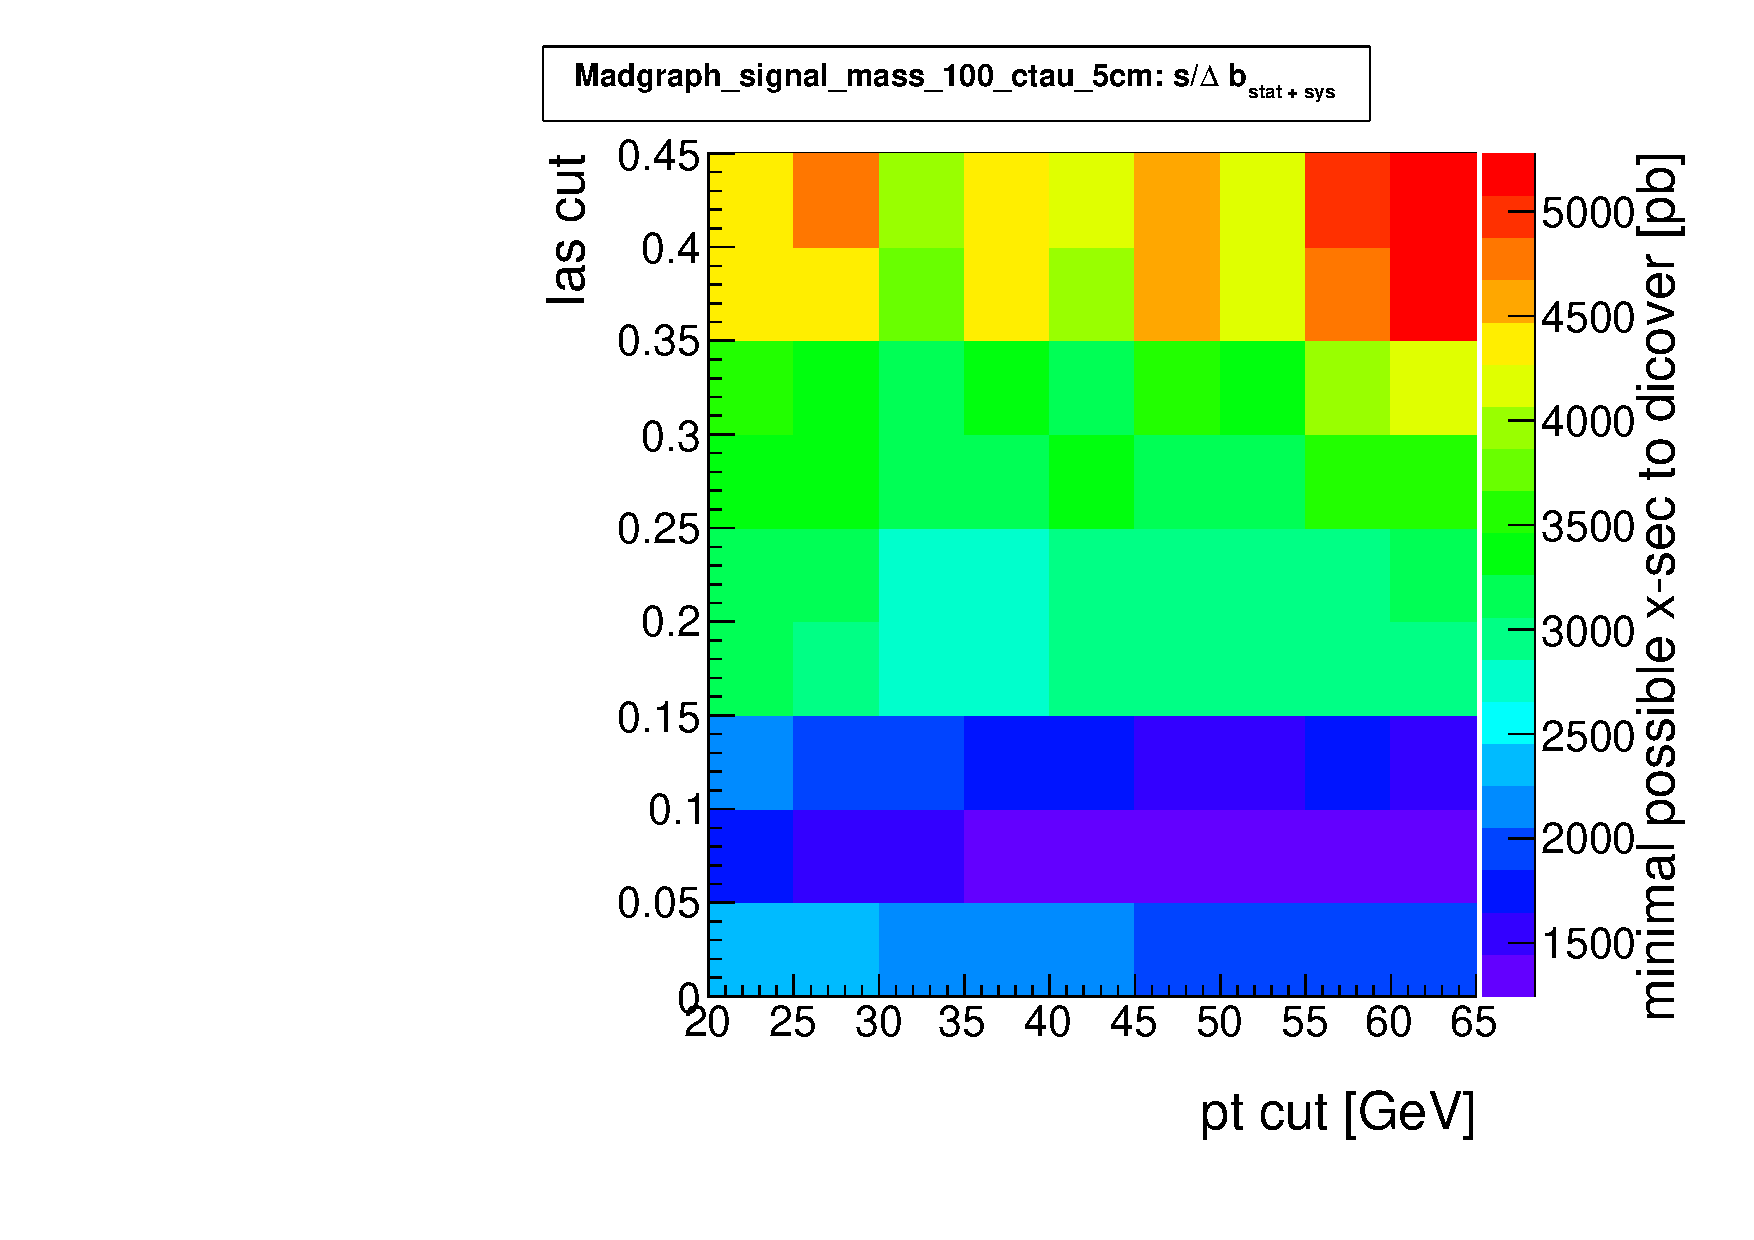
\includegraphics[width=0.49\textwidth]{figures/analysis/Optimisation/Madgraph_signal_mass_100_ctau_5cm_ECaloLe5_SOverDeltaBStatPlusSys.pdf} 
    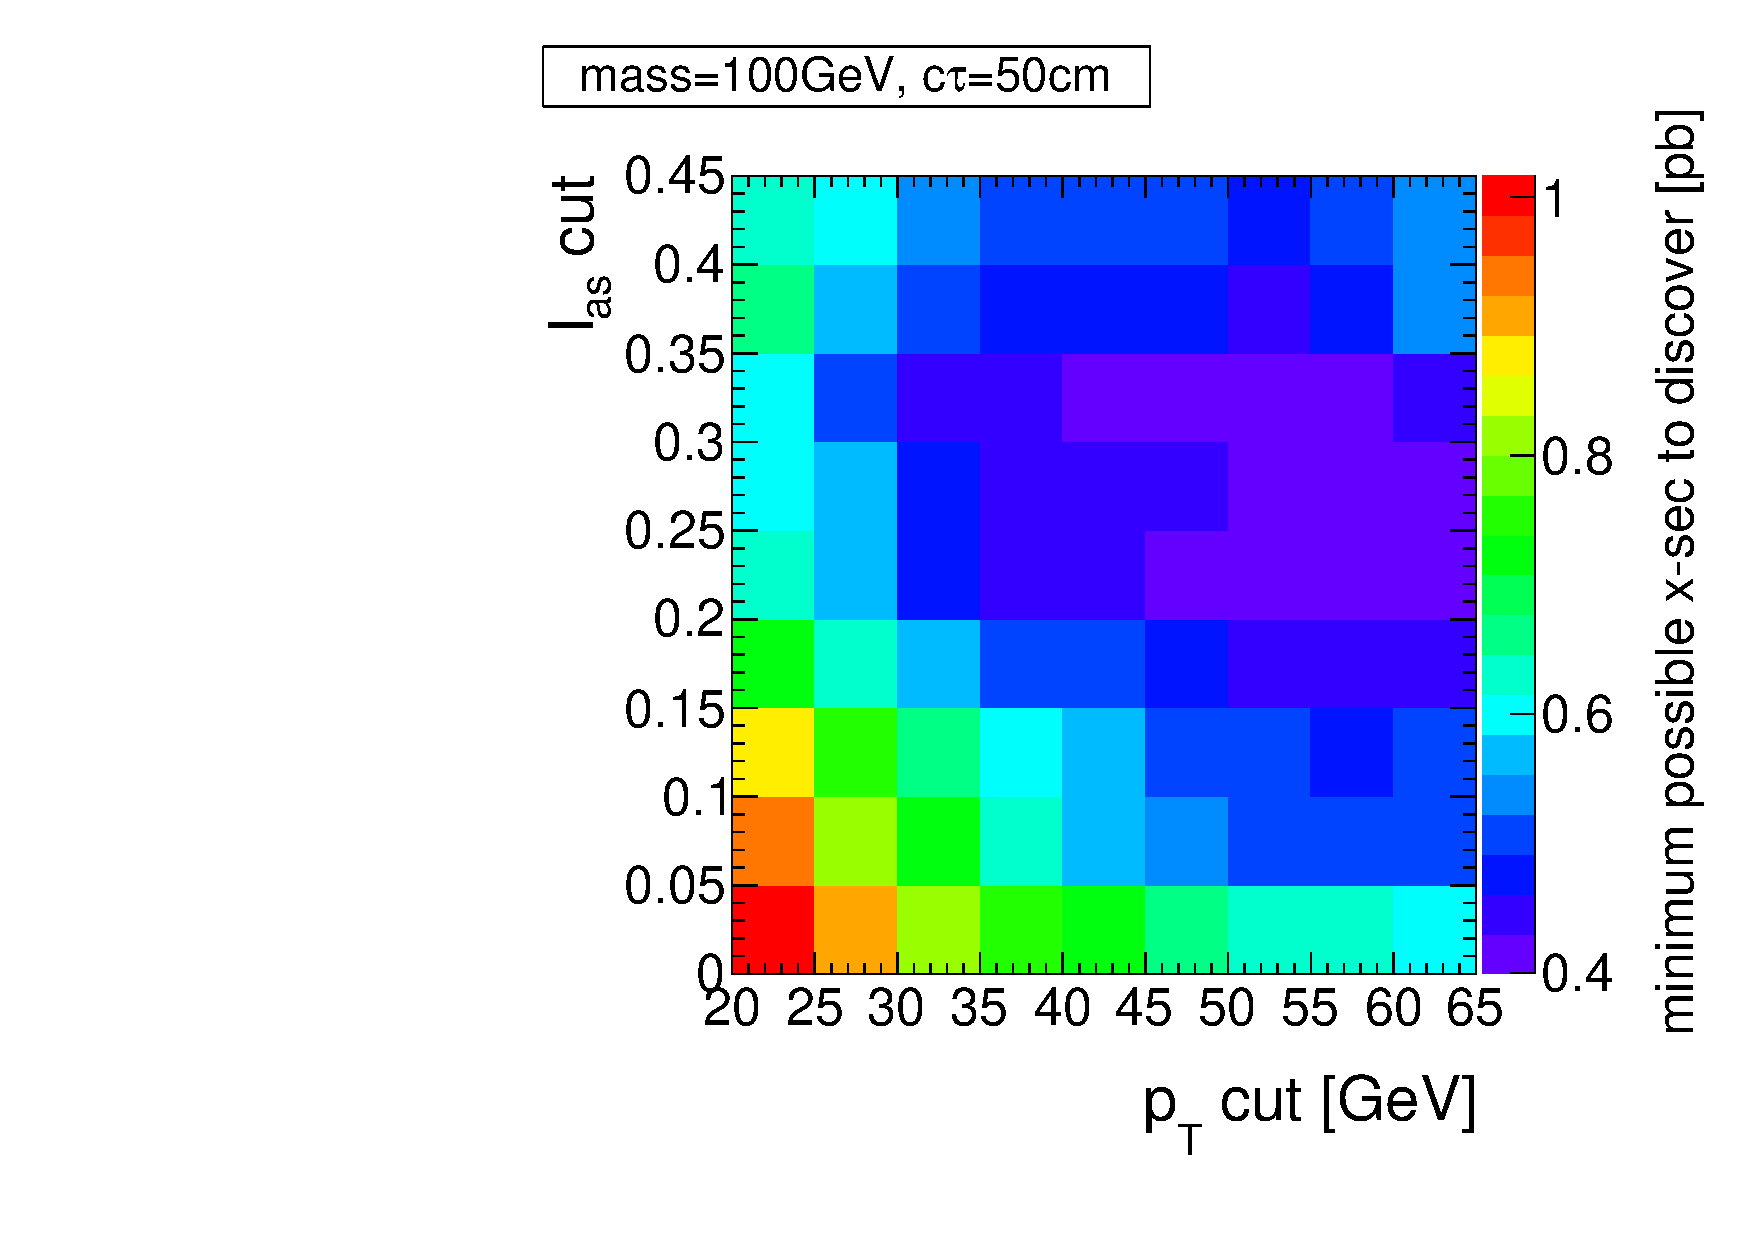
\includegraphics[width=0.49\textwidth]{figures/analysis/Optimisation/Madgraph_signal_mass_100_ctau_50cm_ECaloLe5_SOverDeltaBStatPlusSys.pdf}\\ 
    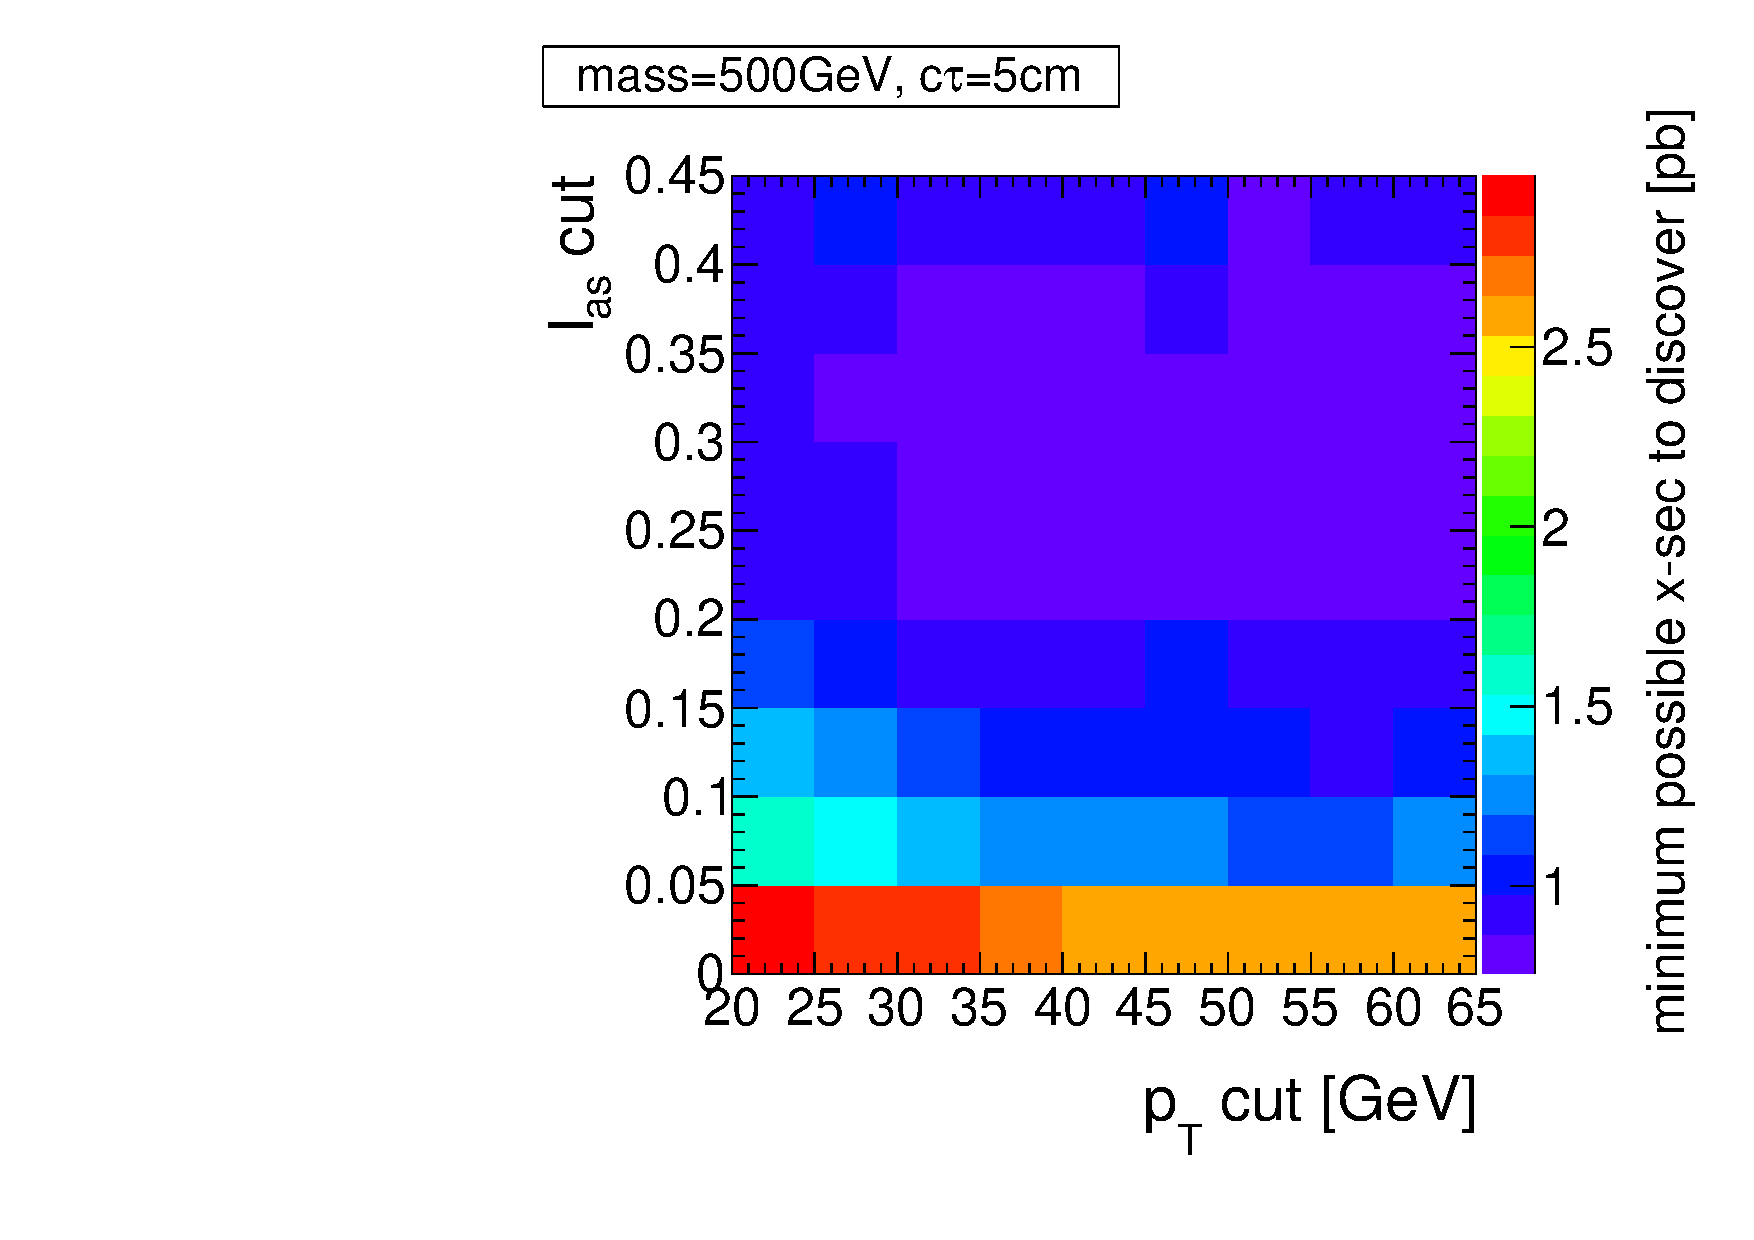
\includegraphics[width=0.49\textwidth]{figures/analysis/Optimisation/Madgraph_signal_mass_500_ctau_5cm_ECaloLe5_SOverDeltaBStatPlusSys.pdf}
    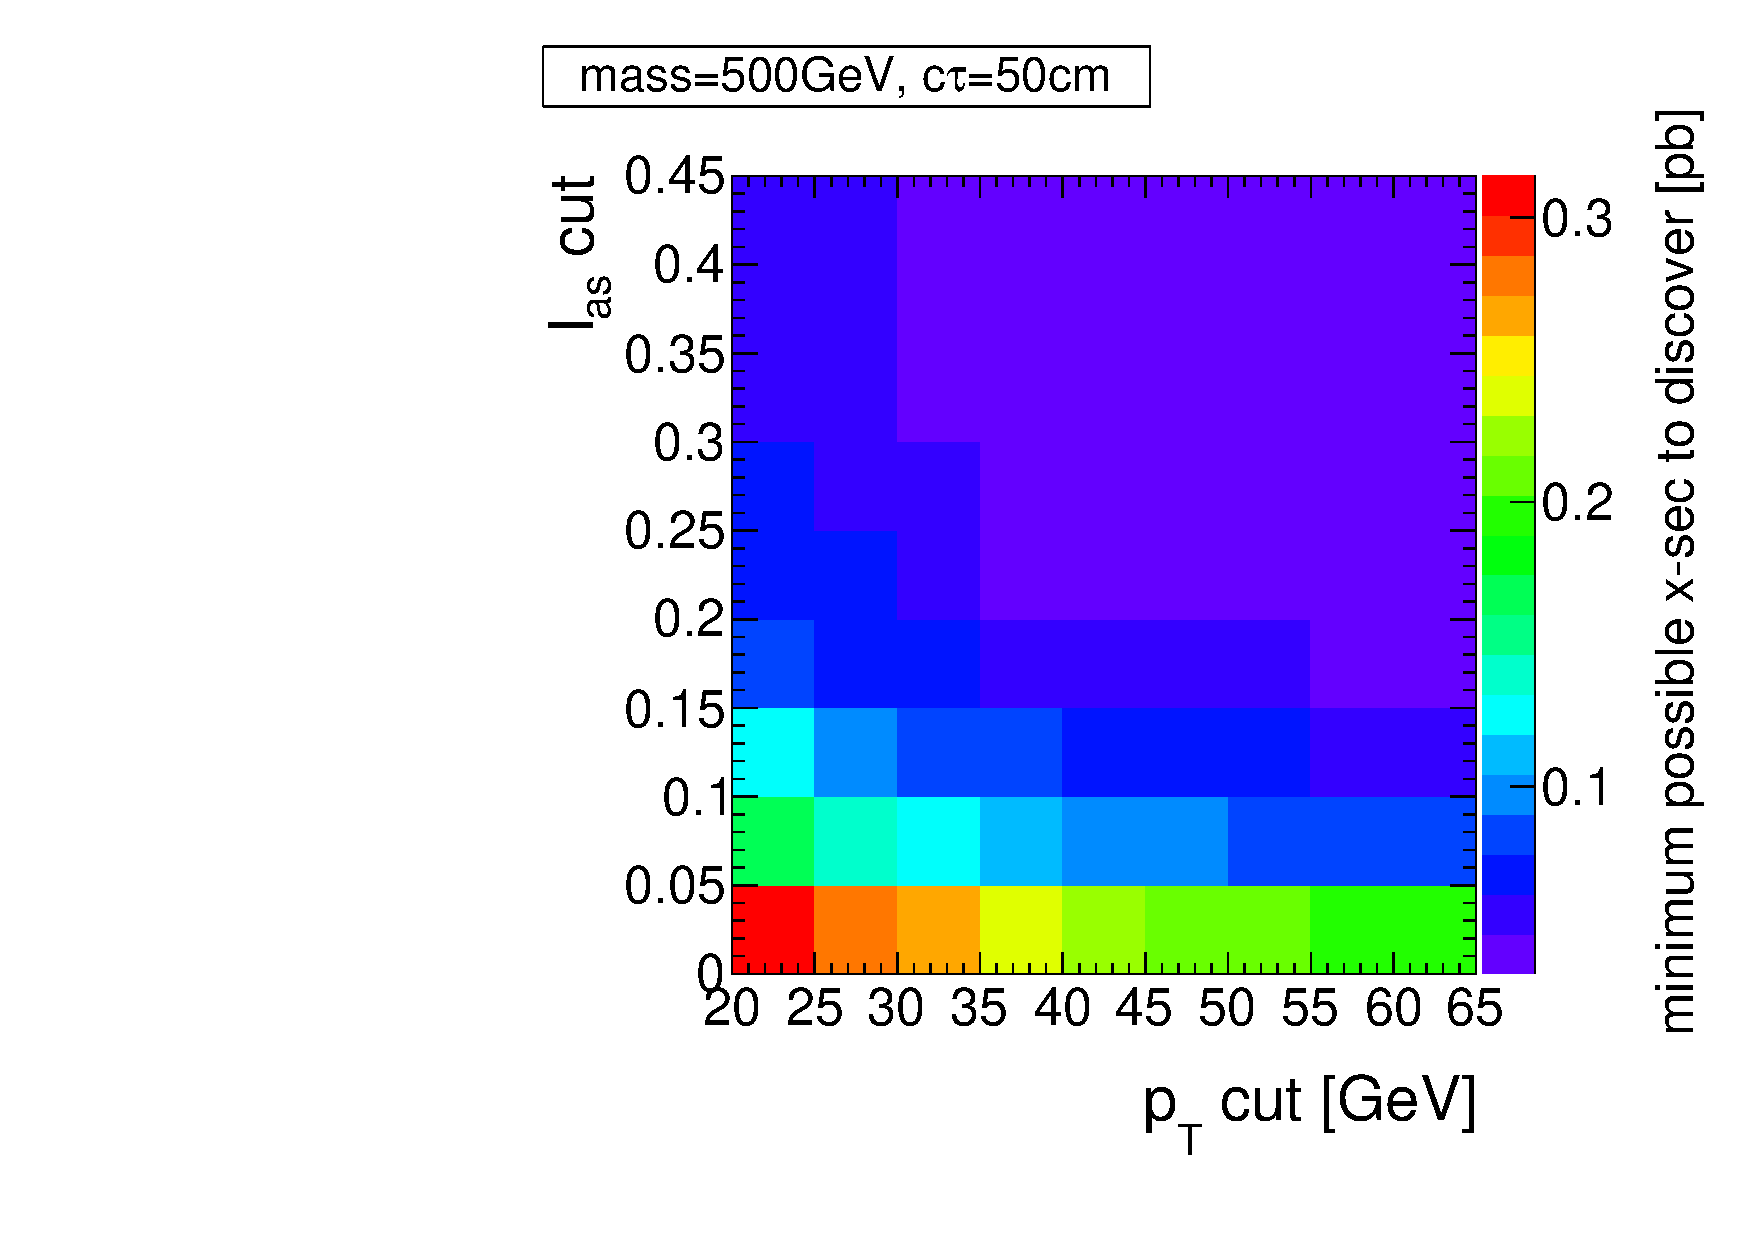
\includegraphics[width=0.49\textwidth]{figures/analysis/Optimisation/Madgraph_signal_mass_500_ctau_50cm_ECaloLe5_SOverDeltaBStatPlusSys.pdf} 
  \end{tabular}
  \caption{Minimum possible cross section that can be discovered with 5$\sigma$ significance in the $\ias-\pt$ plane for four different signal models.
           The systematic uncertainties are taken to be 20\% and 100\% for the fake and the leptonic background respectively.
           The uncertainty on the background arising from the limited size of the used samples are propagated consistently to the search optimisation.
           In Table~\ref{fig:optimisationApp} of Appendix~\ref{app:OptimisationApp}, the corresponding histograms of the background yield, the background uncertainty and the signal yield for the four signal models can be found.}
  \vspace{30pt}
  \label{fig:optimisation}
\end{figure} 
It can be seen, that for low masses and low lifetimes, the highest search sensitivity is achieved by imposing rather soft selection cuts on \ias and \pt.
Optimising for higher lifetime pushes the optimal selection in \pt and \ias to larger values, where signal models with higher masses prefer even tighter \ias selection cuts than the corresponding lower mass signal model.
It can also be seen, that for low lifetimes, the \pt dependence of the search sensitivity is less pronounced than for long lifetimes.\\

For a structured optimisation all background uncertainties as estimated in Section~\ref{sec:SysUncertaintiesBkg} are taken precisely into account. 
As this analysis focus on short tracks, only low lifetimes are considered in the optimisation procedure: $\ctau=1\cm-10\cm$.
To cover the full mass space, the optimisation is done for masses between 100\gev and 500\gev.
The corresponding results are shown in Table~\ref{tab:optimisation}.
\renewcommand{\arraystretch}{1.3}
\begin{table}[!h]
\centering
\caption{Optimal \pt and \ias selection cuts and the corresponding minimum cross section $\sigma_{\text{min}}$ that can be discovered with 5$\sigma$ significance for different signal models.
         For some signal samples a optimisation result is not available due to the limited size of these samples.}
\label{tab:optimisation}
\makebox[0.99\textwidth]{
\begin{tabular}{c |c| c| c| c}
\multicolumn{5}{c}{} \\
\toprule
Mass [\gev] & Lifetime [\cm] & Optimal \pt cut & Optimal \ias cut & $\sigma_{\text{min}}$ \\
\midrule
100&                          1&                            30&                           0.05&                         59.03\\
200&                          1&                            20&                           0.05&                         42.01\\
300&                          1&                            n/a&                          n/a&                          n/a\\
400&                          1&                            n/a&                          n/a&                          n/a\\
500&                          1&                            n/a&                          n/a&                          n/a\\
%600&                          1&                            n/a&                          n/a&                          n/a\\
100&                          5&                            50&                           0.05&                         2.70\\
200&                          5&                            30&                           0.30&                         1.81\\
300&                          5&                            50&                           0.30&                         0.85\\
400&                          5&                            50&                           0.30&                         0.83\\
500&                          5&                            50&                           0.30&                         0.62\\
%600&                          5&                            50&                           0.30&                         0.72\\
100&                          10&                           30&                           0.30&                         1.44\\
200&                          10&                           50&                           0.30&                         0.42\\
300&                          10&                           50&                           0.30&                         0.27\\
400&                          10&                           50&                           0.30&                         0.19\\
500&                          10&                           50&                           0.30&                         0.15\\
%600&                          10&                           50&                           0.30&                         0.14\\
\bottomrule
\multicolumn{5}{c}{} \\
\end{tabular}}
\end{table}

It can be seen that the optimal selection is highly dependent on the signal models.
As in the qualitative optimisation procedure, the search sensitivity for low masses ($\leq 200\gev$) is achieved by soft selection cuts in \pt between $20-30\gev$.
For low lifetimes also the optimal \ias selection cut is soft ($0.05$).
The search sensitivity can be increased in the low mass region for long lifetimes when tightening the \ias selection to a value of 0.3.

For high masses the highest search sensitivity can be achieved with a tighter \pt selection cut of 50\gev and a \ias selection cut of 0.3.


To have an optimal coverage over a wide mass space and a sensitivity reach for different lifetimes, four different exclusive signal regions are defined:
\begin{enumerate}[1.)]
\item $30\gev<\pt<50\gev$ and $0.05<\ias<0.3$
\item $\pt>50\gev$ and $0.05<\ias<0.3$
\item $30\gev<\pt<50\gev$ and $\ias>0.3$
\item $\pt>50\gev$ and $\ias>0.3$.\\
\end{enumerate}

Besides the optimisation in \ias and \pt, is is also checked whether a sensitivity increase can be achieved by imposing also a selection on the number of missing outer hits $N_{\text{lost}}^{\text{outer}}$.
For low lifetimes, a tiny increase in sensitivity of the order of 1-3\% is possible by a $N_{\text{lost}}^{\text{outer}}>0$ selection.
However, as this variable means also a new source of uncertainty on the signal model, such a selection cut is not considered.\\

The next section shows the comparison of the predicted number of events from Standard Model sources to the observed number of events measured in data.

%%%%%%%%%%%%%%%%%%%%%%%%%%%%%%%%%%%%%%%%%%%%%%%%%%%%%%%%%%%%%%%%%%%%%%%%%%%%%%%%%%%%%%%%%%%%%%%%%%%%%%%%%%%%%%%%%%%%%%%%%%%%%%%%%%%%%%%%%%%%%%%%%%%%%%%%%%%%%%%%%%%%%%%
%%%%%%%%%%%%%%%%%%%%%%%%%%%%%%%%%%%%%%%%%%%%%%%%%%%%%%%%%%%%%%%%%%%%%%%%%%%%%%%%%%%%%%%%%%%%%%%%%%%%%%%%%%%%%%%%%%%%%%%%%%%%%%%%%%%%%%%%%%%%%%%%%%%%%%%%%%%%%%%%%%%%%%%
\chapter{Results}
\label{sec:Results}

After developing the methods of the background estimation for all different background sources and their corresponding systematic uncertainties (all explained in Section~\ref{sec:BackgroundEstimation}), 
the search is performed in four exclusive signal regions with 19.7\fbinv of data collected at a centre-of-mass energy of $\sqrt{s} = 8\tev$ at the CMS experiment.
The predicted number of events for the fake and the leptonic background in the four signal regions is depicted in Table~\ref{tab:BackgroundPrediction}.
\renewcommand{\arraystretch}{1.5}
\begin{table}[!h]
\centering
\caption{Background prediction in the four exclusive signal regions for the fake and the leptonic background.}
\label{tab:BackgroundPrediction}
\makebox[0.99\textwidth]{
\begin{tabular}{l |c| c }
\multicolumn{3}{c}{} \\
\toprule
Signal region                                & Fake Bkg                                             & Leptonic Bkg  \\
\midrule
$\pt: 30-50\gev$ / $\ias:0.05-0.30$          & 19.11 $^{+ 2.61} _{- 2.61}$ (stat) $\pm$ 9.35 (sys)      & 0.00 $^{+ 2.58} _{- 0.00}$ (stat) $\pm$ 0.00 (sys) \\
$\pt: 50-\infty\gev$ / $\ias:0.05-0.30$      & 22.21 $^{+ 3.60} _{- 3.60}$ (stat) $\pm$ 8.78 (sys)      & 2.17 $^{+ 2.99} _{- 1.34}$ (stat) $\pm$ 1.65 (sys) \\
$\pt: 30-50\gev$ / $\ias:0.30-1.00$          & 2.49 $^{+ 0.85} _{- 0.85}$ (stat) $\pm$ 1.98 (sys)       & 0.00 $^{+ 0.22} _{- 0.00}$ (stat) $\pm$ 0.00 (sys) \\
$\pt: 50-\infty\gev$ / $\ias:0.30-1.00$      & 2.52 $^{+ 1.14} _{- 1.14}$ (stat) $\pm$ 1.27 (sys)       & 0.04 $^{+ 0.30} _{- 0.03}$ (stat) $\pm$ 0.03 (sys) \\
\bottomrule
\multicolumn{3}{c}{}\\
\end{tabular}}
\end{table}
It can be seen, that fake tracks are by far the dominant background to this search.
The leptonic background contributes only in one signal region to the total background with a share of about 10\%.

Finally, the comparison between the predicted number of events and the number of observed events is shown in Fig.~\ref{fig:FinalResult}.
\begin{figure}[!t]
  \centering 
  \begin{tabular}{c}
    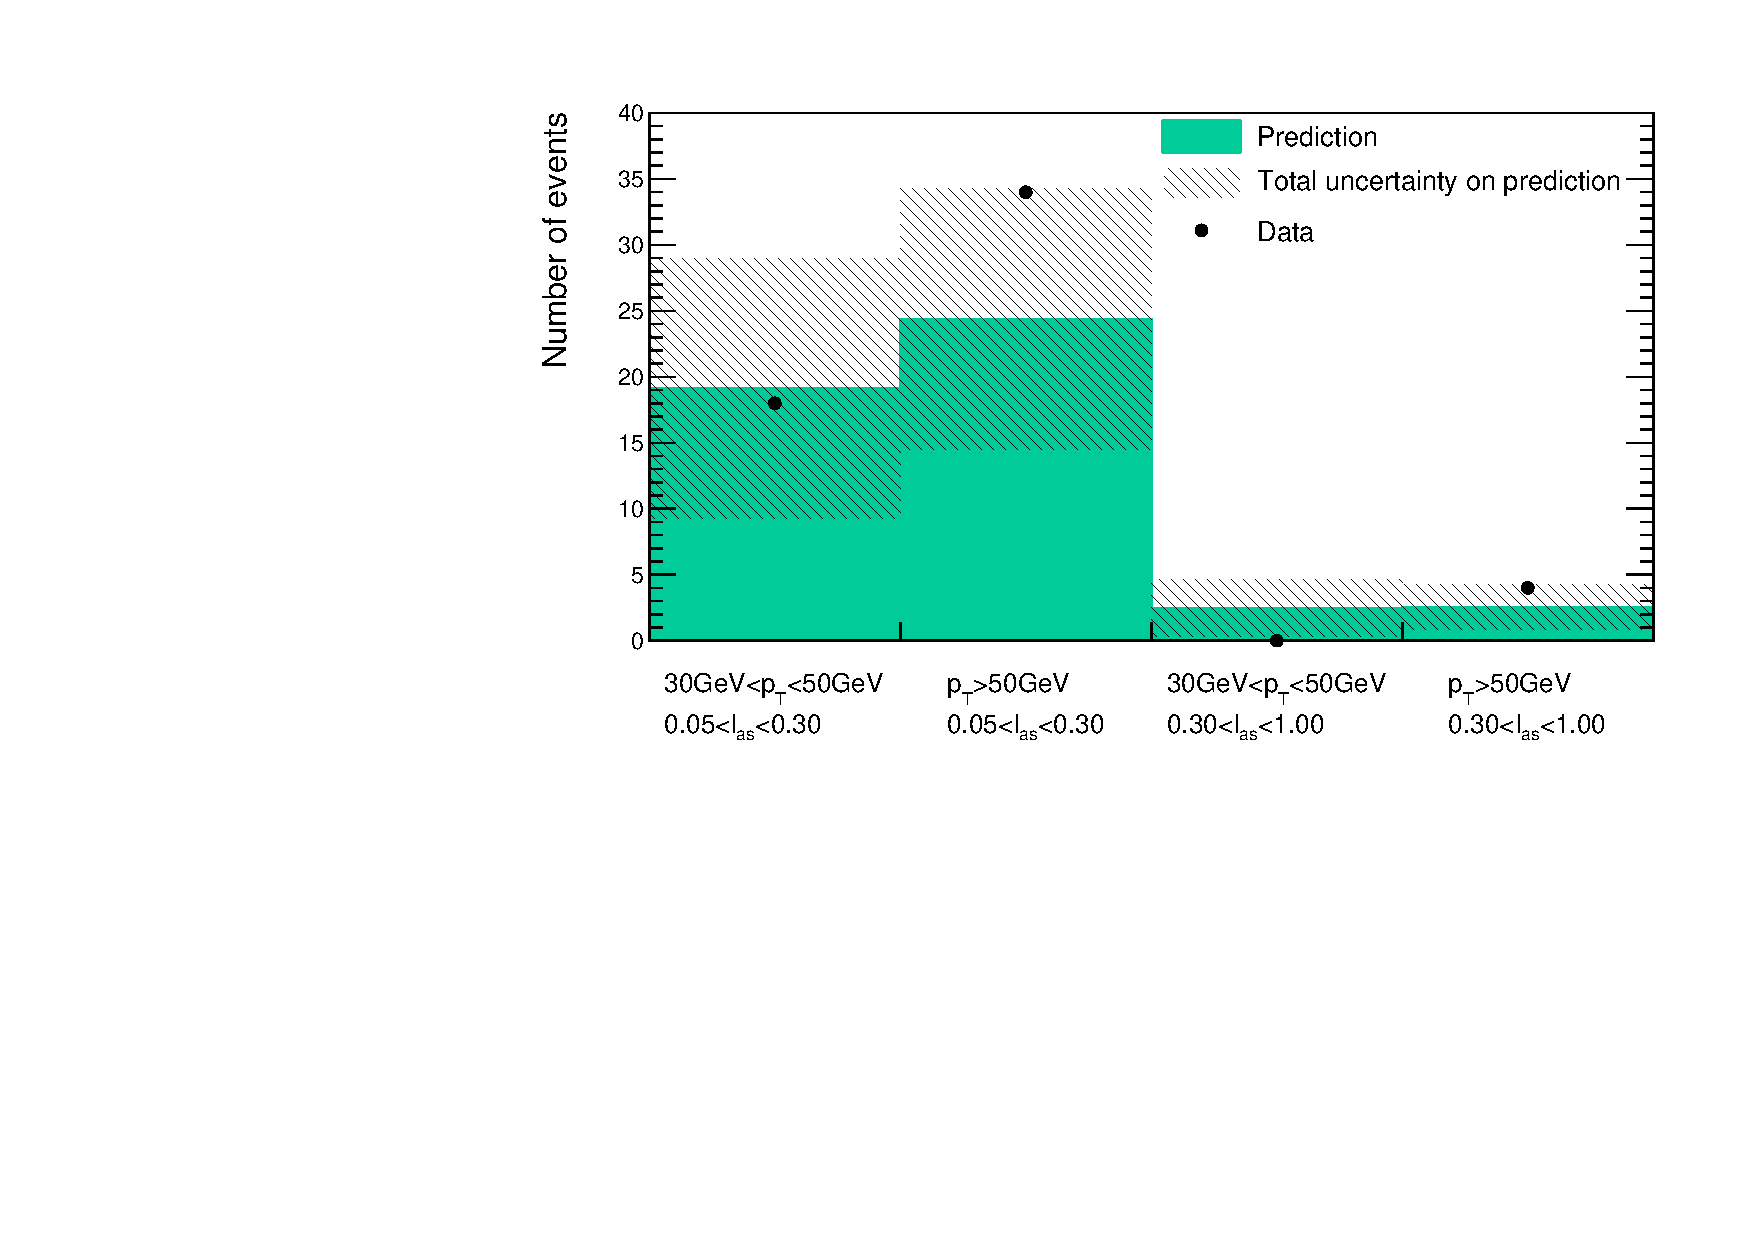
\includegraphics[width=0.99\textwidth]{figures/analysis/Results/FinalResultPlot.pdf} 
  \end{tabular}
  \caption{Number of predicted (green area) and observed (black dots) events for the four different signal regions. The hashed area represents the total uncertainty on the background prediction.}
  \label{fig:FinalResult}
 \vspace{50pt}
\end{figure} 
Additionally, the corresponding numbers of predicted and observed events can be found in Table~\ref{tab:FinalResult}.
\renewcommand{\arraystretch}{1.5}
\begin{table}[!h]
\centering
\caption{Number of predicted and observed events for the four different signal regions.}
\label{tab:FinalResult}
\makebox[0.99\textwidth]{
\begin{tabular}{l |c| c}
\multicolumn{3}{c}{} \\
\toprule
Signal region                         & Prediction                                              & Observation  \\
\midrule
$\pt: 30-50\gev$ / $\ias:0.05-0.30$      & 19.11 $^{+ 3.67} _{- 2.61}$ (stat) $\pm$ 9.35 (sys)         & 18           \\
$\pt: 50-\infty\gev$ / $\ias:0.05-0.30$  & 24.38 $^{+ 4.68} _{- 3.84}$ (stat) $\pm$ 8.93 (sys)         & 34           \\
$\pt: 30-50\gev$ / $\ias:0.30-1.00$     & 2.49 $^{+ 0.87} _{- 0.85}$ (stat) $\pm$ 1.98 (sys)          & 0            \\
$\pt: 50-\infty\gev$ / $\ias:0.30-1.00$ & 2.57 $^{+ 1.18} _{- 1.14}$ (stat) $\pm$ 1.27 (sys)          & 4            \\
\bottomrule
\multicolumn{3}{c}{} \\
\end{tabular}}
\end{table}
The event yields observed in data after each selection requirement for the four signal regions are listed in Table~\ref{FIXME} in Appendix~\ref{FIXME}.

The results are compatible in all four signal regions with the Standard Model background within the 1$\sigma$ uncertainties.
No excess above the SM prediction is in either of the four signal regions observed.
Thus, no evidence for physics beyond the Standard Model could be found.

Therefore, in the following section the result will be interpreted within the context of a supersymmetric models with wino-like charginos and neutralinos.
%\renewcommand{\arraystretch}{1.5}
%\begin{table}[!h]
%\centering
%\caption{Background prediction from the four different background sources: Fakes, taus, muons and electrons.}
%\label{tab:FinalResult}
%\makebox[0.99\textwidth]{
%\begin{tabular}{l |c| c | c| c}
%\multicolumn{3}{c}{} \\
%\toprule
%Signal region                         & Fakes   & Taus  & Muons & Electrons  \\
%\midrule
%$30\gev<\pt<50\gev$ / $0.05<\ias<0.3$ & 19.11 $^{+ 2.61} _{- 2.61}$ (stat) $\pm$ 9.35 (sys)      & 0.00 $^{+ 0.87} _{- 0.00}$ (stat) $\pm$ 0.00 (sys) & 0.00 $^{+ 0.22} _{- 0.00}$ (stat) $\pm$ 0.00 (sys) & 0.00 $^{+ 2.42} _{- 0.00}$ (stat) $\pm$ 0.00 (sys)                           \\
%$\pt>50\gev$        / $0.05<\ias<0.3$ & 22.21 $^{+ 3.60} _{- 3.60}$ (stat) $\pm$ 8.78 (sys)      & 0.00 $^{+ 0.33} _{- 0.00}$ (stat) $\pm$ 0.00 (sys) & 0.00 $^{+ 0.29} _{- 0.00}$ (stat) $\pm$ 0.00 (sys) & 2.17 $^{+ 2.96} _{- 1.34}$ (stat) $\pm$ 1.65 (sys)                             \\
%$30\gev<\pt<50\gev$ / $\ias>0.3$      & 2.49 $^{+ 0.85} _{- 0.85}$ (stat) $\pm$ 1.98 (sys)       & 0.00 $^{+ 0.01} _{- 0.00}$ (stat) $\pm$ 0.00 (sys) & 0.00 $^{+ 0.22} _{- 0.00}$ (stat) $\pm$ 0.00 (sys) & 0.00 $^{+ 0.05} _{- 0.00}$ (stat) $\pm$ 0.00 (sys)                      \\
%$\pt>50\gev$        / $\ias>0.3$      & 2.52 $^{+ 1.14} _{- 1.14}$ (stat) $\pm$ 1.27 (sys)       & 0.00 $^{+ 0.00} _{- 0.00}$ (stat) $\pm$ 0.00 (sys) & 0.00 $^{+ 0.29} _{- 0.00}$ (stat) $\pm$ 0.00 (sys) & 0.04 $^{+ 0.06} _{- 0.03}$ (stat) $\pm$ 0.03 (sys)                      \\
%\bottomrule
%\multicolumn{3}{c}{} \\
%\end{tabular}}
%\end{table}






%%%%%%%%%%%%%%%%%%%%%%%%%%%%%%%%%%%%%%%%%%%%%%%%%%%%%%%%%%%%%%%%%%%%%%%%%%%%%%%%%%%%%%%%%%%%%%%%%%%%%%%%%%%%%%%%%%%%%%%%%%%%%%%%%%%%%%%%%%%%%%%%%%%%%%%%%%%%%%%%%%%%%%%
%%%%%%%%%%%%%%%%%%%%%%%%%%%%%%%%%%%%%%%%%%%%%%%%%%%%%%%%%%%%%%%%%%%%%%%%%%%%%%%%%%%%%%%%%%%%%%%%%%%%%%%%%%%%%%%%%%%%%%%%%%%%%%%%%%%%%%%%%%%%%%%%%%%%%%%%%%%%%%%%%%%%%%%
\newpage
\chapter{Interpretation}
\label{sec:Interpretation}
In order to interpret the result of the search in the context of supersymmetric models with wino-like charginos and neutralinos, sources of systematic uncertainties on the number of selected signal events must be identified
and their size must be estimated.
Furthermore, the size of correlations between the systematic uncertainties must be determined to be able to combine the results of all four signal regions.
The interpretation will then be done with statistical methods, that allow for the exclusion of parts of the supersymmetric parameter space on a 95\% confidence level.

\section{Systematic uncertainties of simulated signal samples}
The systematic uncertainties on the number of signal events in the four signal regions are mainly caused by uncertainties on the quality of the simulation.
This influences the signal efficiency of each selection requirement in this analysis.
Furthermore, an uncertainty on the overall number of events is caused by the uncertainty on the integrated luminosity recorded in 2012 at CMS and the theoretical signal cross-sections.

\subsection*{Luminosity uncertainty}
The integrated luminosity recorded at CMS during the year 2012 is measured with the counting of pixel clusters during the crossing of two bunches (zero-bias event).
A detailed explanation of this method and the corresponding total uncertainty of 2.6\% can be found in \cite{bib:CMS:Lumi_PAS}.

\subsection*{Uncertainty on the theoretical cross section}
The theoretical cross sections of $\chipm\chimp$ and $\chipm\chiO$ production at a centre-of-mass energy of 8\tev are taken from \cite{bib:SignalCrossSection_2012,bib:SignalCrossSection_2013}.
The corresponding theoretical uncertainties are ranging between $3-10\%$.

\subsection*{Uncertainty on the simulation of initial state radiation}
Initial state radiation affects the transverse momentum distribution of the 2-particle system, $\pt\left(p_1^{\mu} + p_2^{\mu} \right)$, in a 2-body decay.
Differences between data and simulation of ISR are taken into account by reweighting the transverse momentum of the $\chipm\chimp$ or $\chipm\chiO$ system.
The weights are determined with a comparison of the simulated and observed \pt distribution of $Z$ and $\bar{t}t$ events, done in~\cite{bib:CMS:ISR_AN}.
To account for the systematic uncertainties on the reweighting procedure, the event weights are varied up and down dependent on the $\pt^{\chi_1\chi_2}$ up to variations of 25\%.
The resulting uncertainty on the ISR simulation is between $10-13\%$.

\subsection*{Uncertainty on the simulation of the trigger efficiency}
The HLTMonoCentralPFJet80\_PFMETnoMu105\_NHEF0p95 trigger with the higher MET threshold of 105\gev active in Run\,C and Run\,D during 2012 was not available in the simulated signal samples.
It is therefore emulated using L1 trigger information. 
More details on the emulation of this trigger can be found in Appendix~\ref{app:TriggerEmulation}.

The trigger uncertainty is accessed by comparing data-simulation differences of the trigger efficiency.
This has been done within~\cite{bib:CMS:DT_Thesis,bib:CMS:DT_8TeV_AN}.
The resulting differences are applied as variations of the event weights of the simulated samples.
The corresponding uncertainty lies between $2.6-4.6\%$ for the signal samples.

\subsection*{Uncertainty on the jet energy scale}
The transverse momentum of all jets is corrected for non-uniformities in the energy response as a function of the jet $\eta$ and \pt~\cite{bib:CMS:JME_PAS} and for data-simulation differences.
The uncertainty on the jet energy scale (JES) arise from the systematic uncertainty of the jet response in data like jet fragmentation, jet flavor composition, etc., neatly described in~\cite{bib:CMS:JME_PAS}.
The correction is applied as a multiplicant on each jet's transverse momentum contained in an event.
The corresponding systematic uncertainty is accessed by a up and down variation of the correction factor within 1\,$\sigma$.
The resulting uncertainties are of minor importance and lie between $0.5-1.1\%$.

\subsection*{Uncertainty on the jet energy resolution}
The jet energy resolution (JER) is smaller in simulation than in measured data (see Part~\ref{FIXME}). 
To take into account these differences, the jet energy response is additionnaly smeared to match the measured response.
The systematic uncertainties cover the uncertainty on the resolution in data, like the jet energy scale uncertainty, uncertainties arising from out-of-cone showering etc.~\cite{bib:CMS:JME_PAS,bib:Kristin_Thesis}.
The resulting uncertainty on the signal efficiency is between $0.1-0.7\%$ and therefore almost negliglbe.

\subsection*{Uncertainty on the simulation of the parton distribution functions}
The parton distribution function (PDF) used for the simulation of proton-proton collisions is provided by the \cteq group~\cite{Pumplin:2002vw} (see Section~\ref{FIXME} for more information about PDFs).
In~\cite{Pumplin:2002vw}, a detailed description of the methodology of the determination of a parton distribution function and its uncertainties is given.
Pratically, the estimation of the PDF uncertainty is done by the application of 44 different sets of event weights which take into account 22 different sources of uncertainties~\cite{Botje:2011sn,bib:PDF_practical} 
(up and down variations lead to a factor of 2).
The sources correspond inter alia to uncertainties in the single distributions of gluons, up/down-quarks, etc, with the gluon distribution being by far the largest source of uncertainty.

The resulting uncertainties on the signal efficiency are between $3-5\%$.

\subsection*{Uncertainty of the pile-up reweighting}
As mentioned before, the distribution of the number of primary vertices is reweighted to match the measured distribution in data.
The number of interactions in data on the other hand is determined by the luminosity of each bunch-crossing times the proton-proton inelastic cross section which is 69.4\mb.
The uncertainty on the number of interactions consists thus out of the uncertainty on the luminosity and the uncertainty on the cross section.
To cover both sources, a variation of the inelastic cross section by plus/minus 5\% is done.

The signal efficiency is only affected with less than 1\% by this sytematic uncertainty.

\subsection*{Uncertainty on the simulation of the calorimeter isolation}
The uncertainty on the simulation of the calorimeter isolation \ecalo is estimated by the comparison of the cut selection efficiency of $\ecalo<5\gev$ in the fake enriched control sample \fakeCR.
The fake enriched control region is well suited for this estimation, as fake tracks are also expected to deposit only a low amount of energy in the calorimeters.
The selection efficiency in data is higher than in simulation in both \pt bins of $30-50\gev$ and $50-\infty\gev$, which results in an uncertainty of 12\% and 3\% respectively.


\subsection*{Uncertainty on the simulation of missing middle/inner hits}
The uncertainty on the simulation of the number of missing inner and middle hits is assessed by comparing the probability of passing the selection requirements of $N_{\text{miss}}^{\text{middle/inner}}=0$
of a candidate track in the muon-veto inverted control region. 
This control region is particulary suitable because muons are neither expected to have intrinsic sources of missing hits, as pions or electrons have.
Pions can interact nuclearly with the tracker material and electrons can have sizeable radiative losses, such that both can change direction or don't deposit energy in a tracker layer.
For muons, on the other hand, sources of missing inner and middle hits are mainly algorithmical~\cite{bib:CMS:DT_Thesis,bib:CMS:DT_8TeV_AN}, 
making them very similar to the algorithmic sources of missing inner/middle hits for chargino tracks.

The uncertainty is estimated as the relative difference of the cut selection efficiency of $N_{\text{miss}}^{\text{middle/inner}}=0$ in data and simulation.
The selection efficiency is always higher in simulation, resulting in systematic uncertainties of around 3.5\% for the simulation of $N_{\text{miss}}^{\text{inner}}=0$ and around 2.0\% for $N_{\text{miss}}^{\text{middle}}=0$.
The uncertainties are of very similar size in the signal regions with different \pt.
No \ias dependence is considered.

\subsection*{Uncertainty on the simulation of \ias}
An uncertainty on the simulation of \ias needs to be estimated to account for possible data-simulation differences for highly ionising particles.
The estimation of the \ias uncertainty is done as in~\cite{bib:CMS:HSCP_8TeV,bib:CMS:HSCP_8TeV_AN}.
The \ias uncertainty can be assessed by comparing data and simulation differences of slow protons.
Slow protons are highly ionising, thus, can be used to determine the uncertainty in the high \ias region.

%The estimation is done with the ``Minimum Bias'' samples also used for the pixel calibration (see Section~\ref{sec:EnergyCalibration}).
In order to select slow protons, good quality tracks with a momentum smaller than 2.5\gev are selected.
The \ias versus momentum distribution for the selected tracks are shown in Fig.~\ref{fig:IasVsMomentum}.
The kaon, proton and in data also the deuteron line is visible.
\begin{figure}[!h]
  \centering 
  \begin{tabular}{c}
    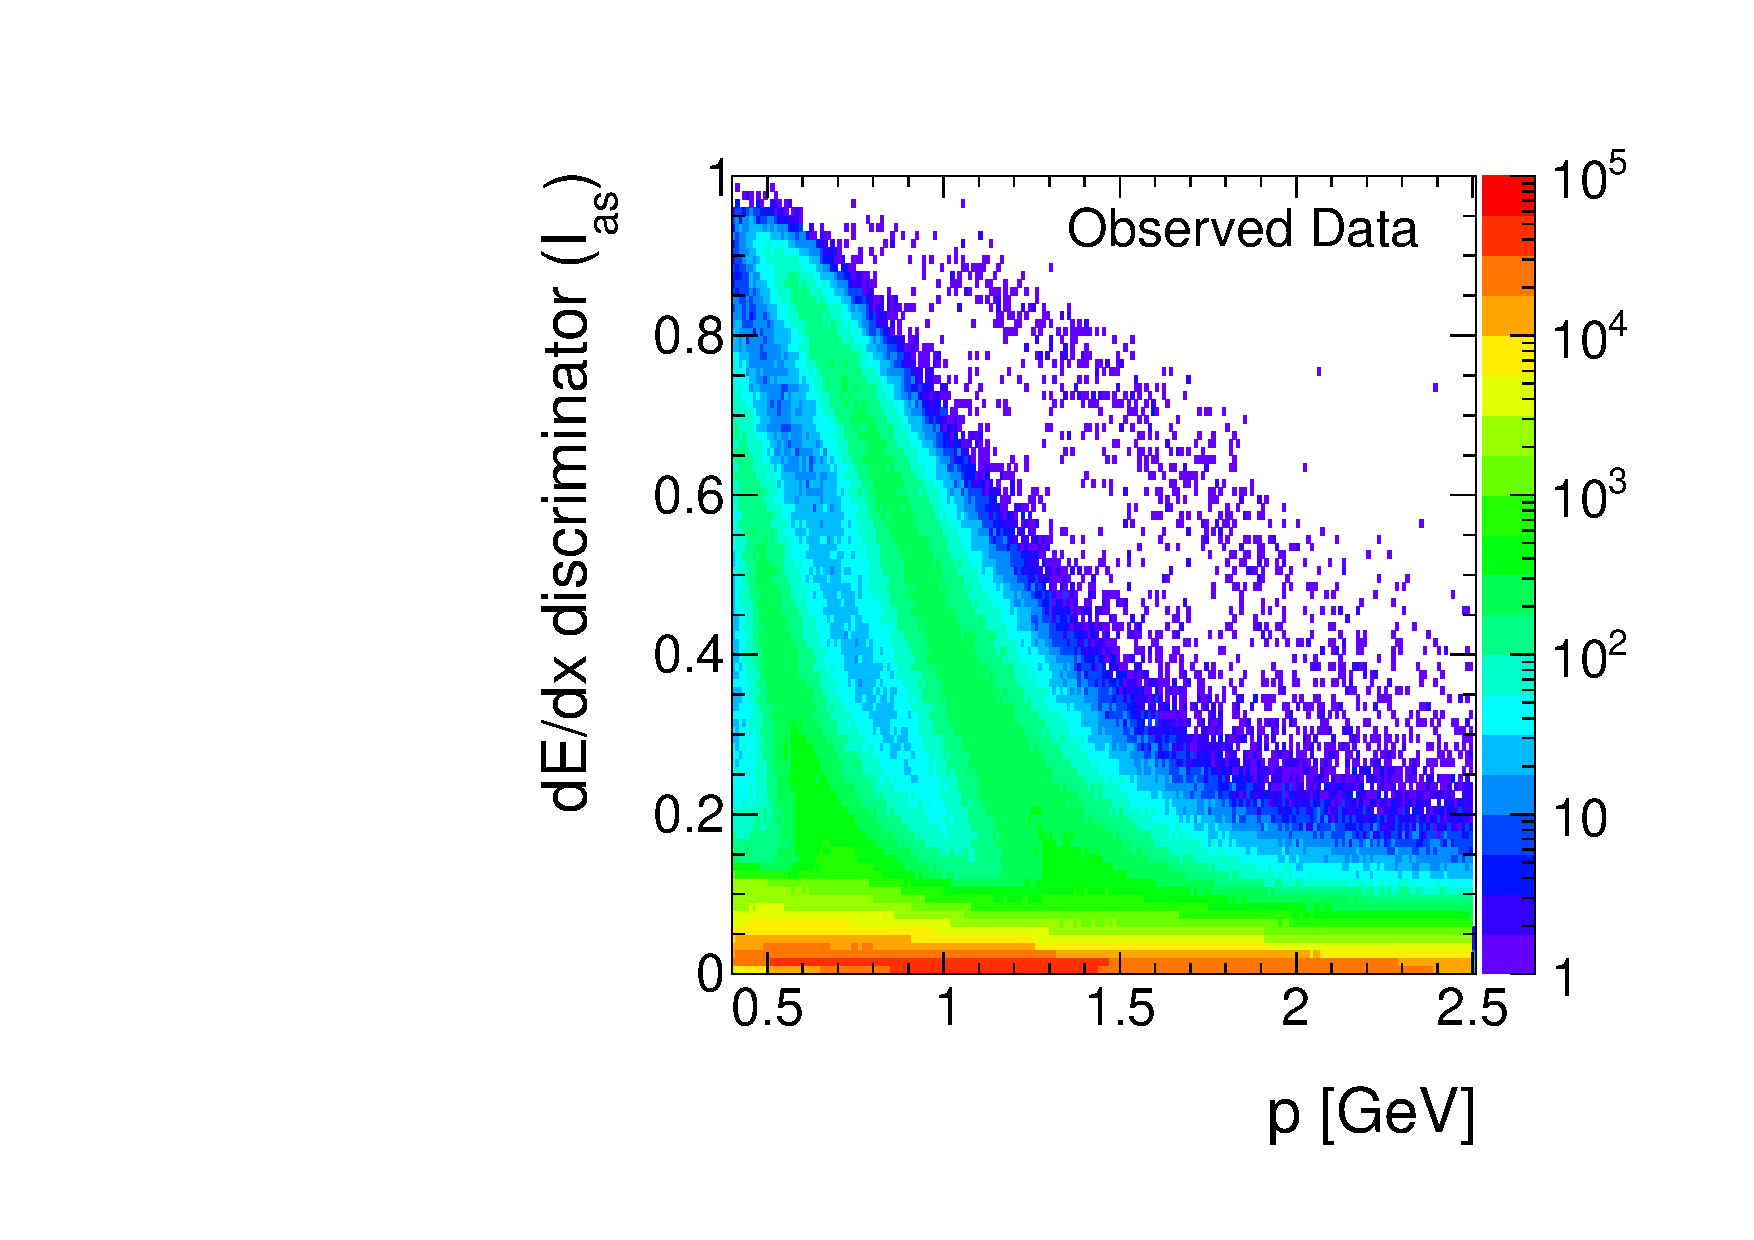
\includegraphics[width=0.49\textwidth]{figures/analysis/Interpretation/IasP_Data.pdf} 
    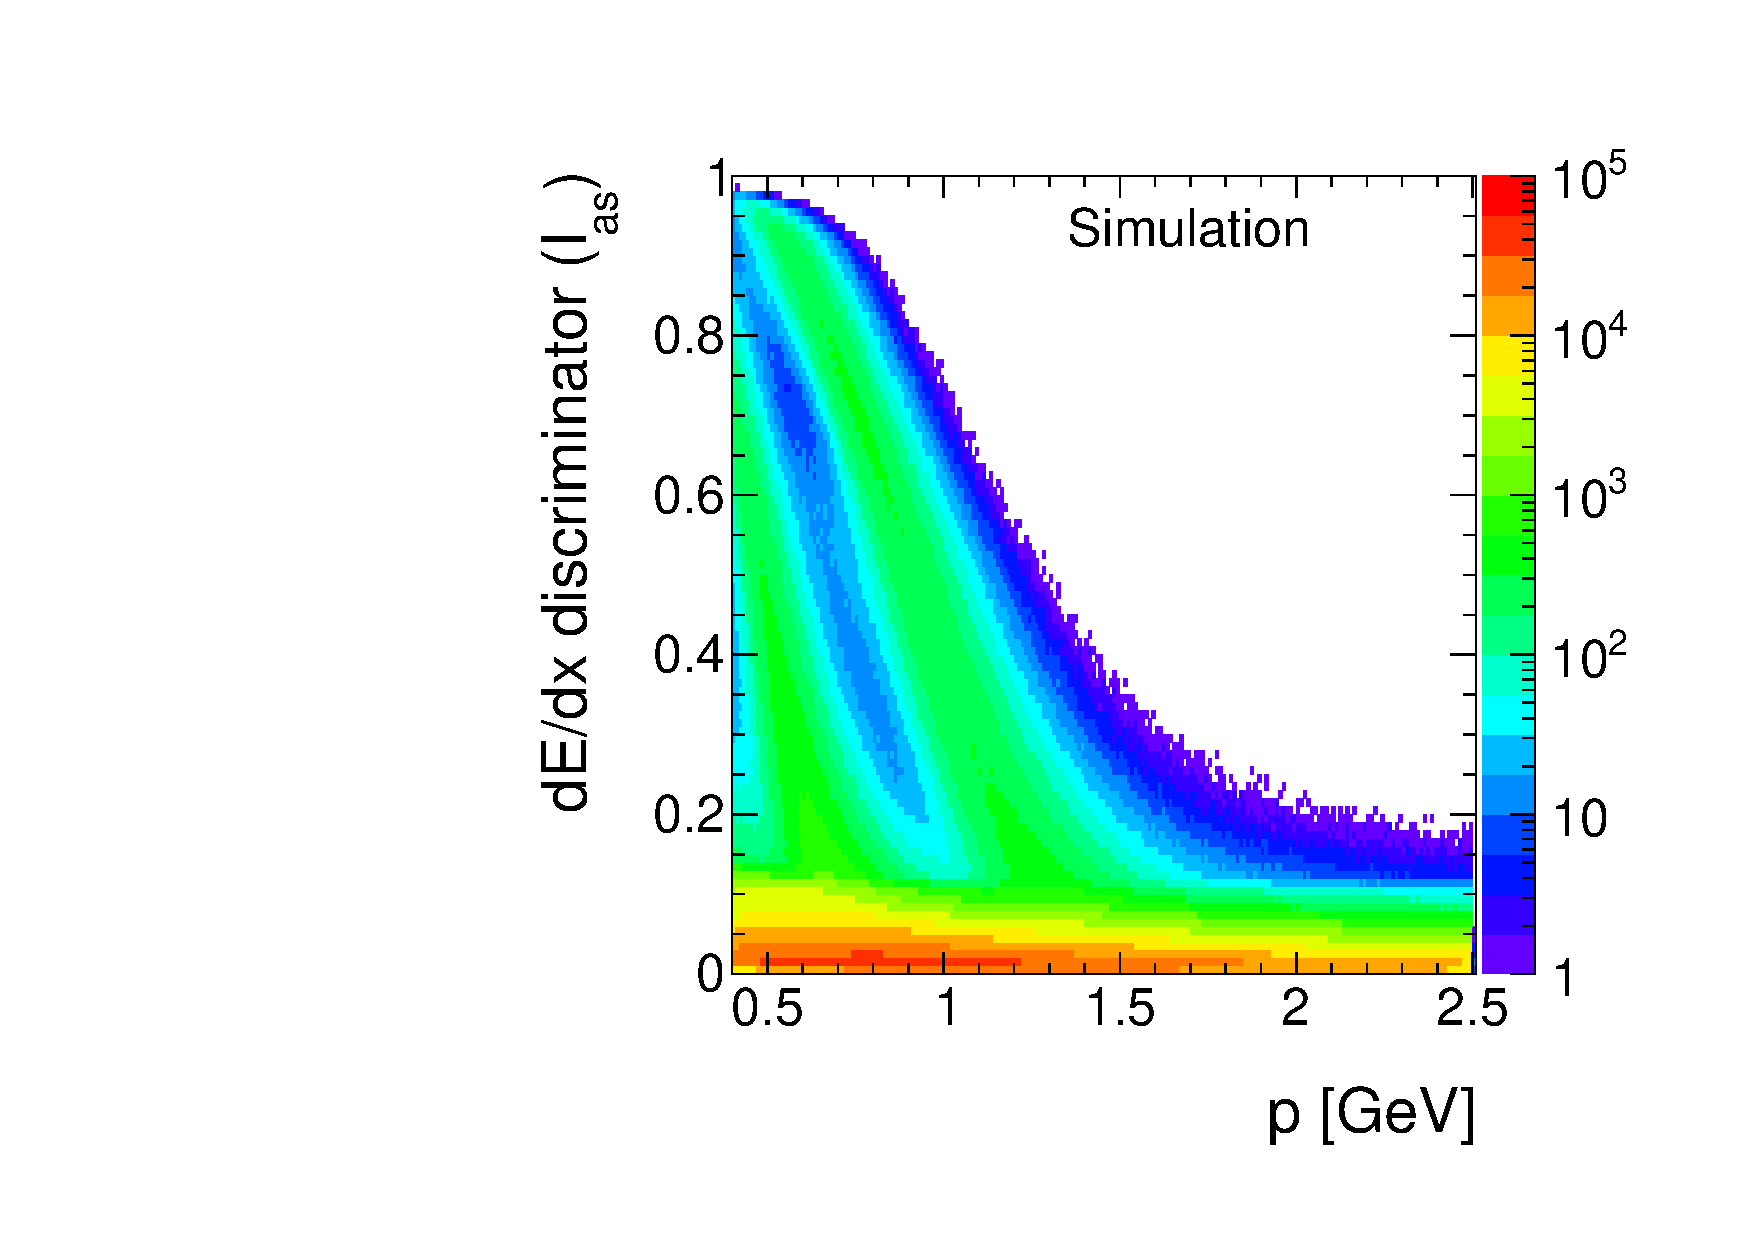
\includegraphics[width=0.49\textwidth]{figures/analysis/Interpretation/IasP_MC.pdf}
  \end{tabular}
  \caption{\ias versus momentum for good quality tracks with at least eight hits in observed data (left) and simulation (right).
           The kaon and proton line are visible in both datasets. The deuteron line is only visible in data, as deuterons are not simulated.}
  \label{fig:IasVsMomentum}
\end{figure} 
Two different slices in the momentum are extracted where the proton line is contained: p between $0.80-0.85$ and $0.95-1.00$.
A gaussian function is fitted to the proton peak and the maximal difference of the mean the fitted gaussian between simulation and observed data is taken as systematic uncertainty.
The \ias distribution for the two momentum ranges with the Gaussian fit is depicted in Fig.~\ref{fig:IasSlowProtons}.
\begin{figure}[!h]
  \centering 
  \begin{tabular}{c}
    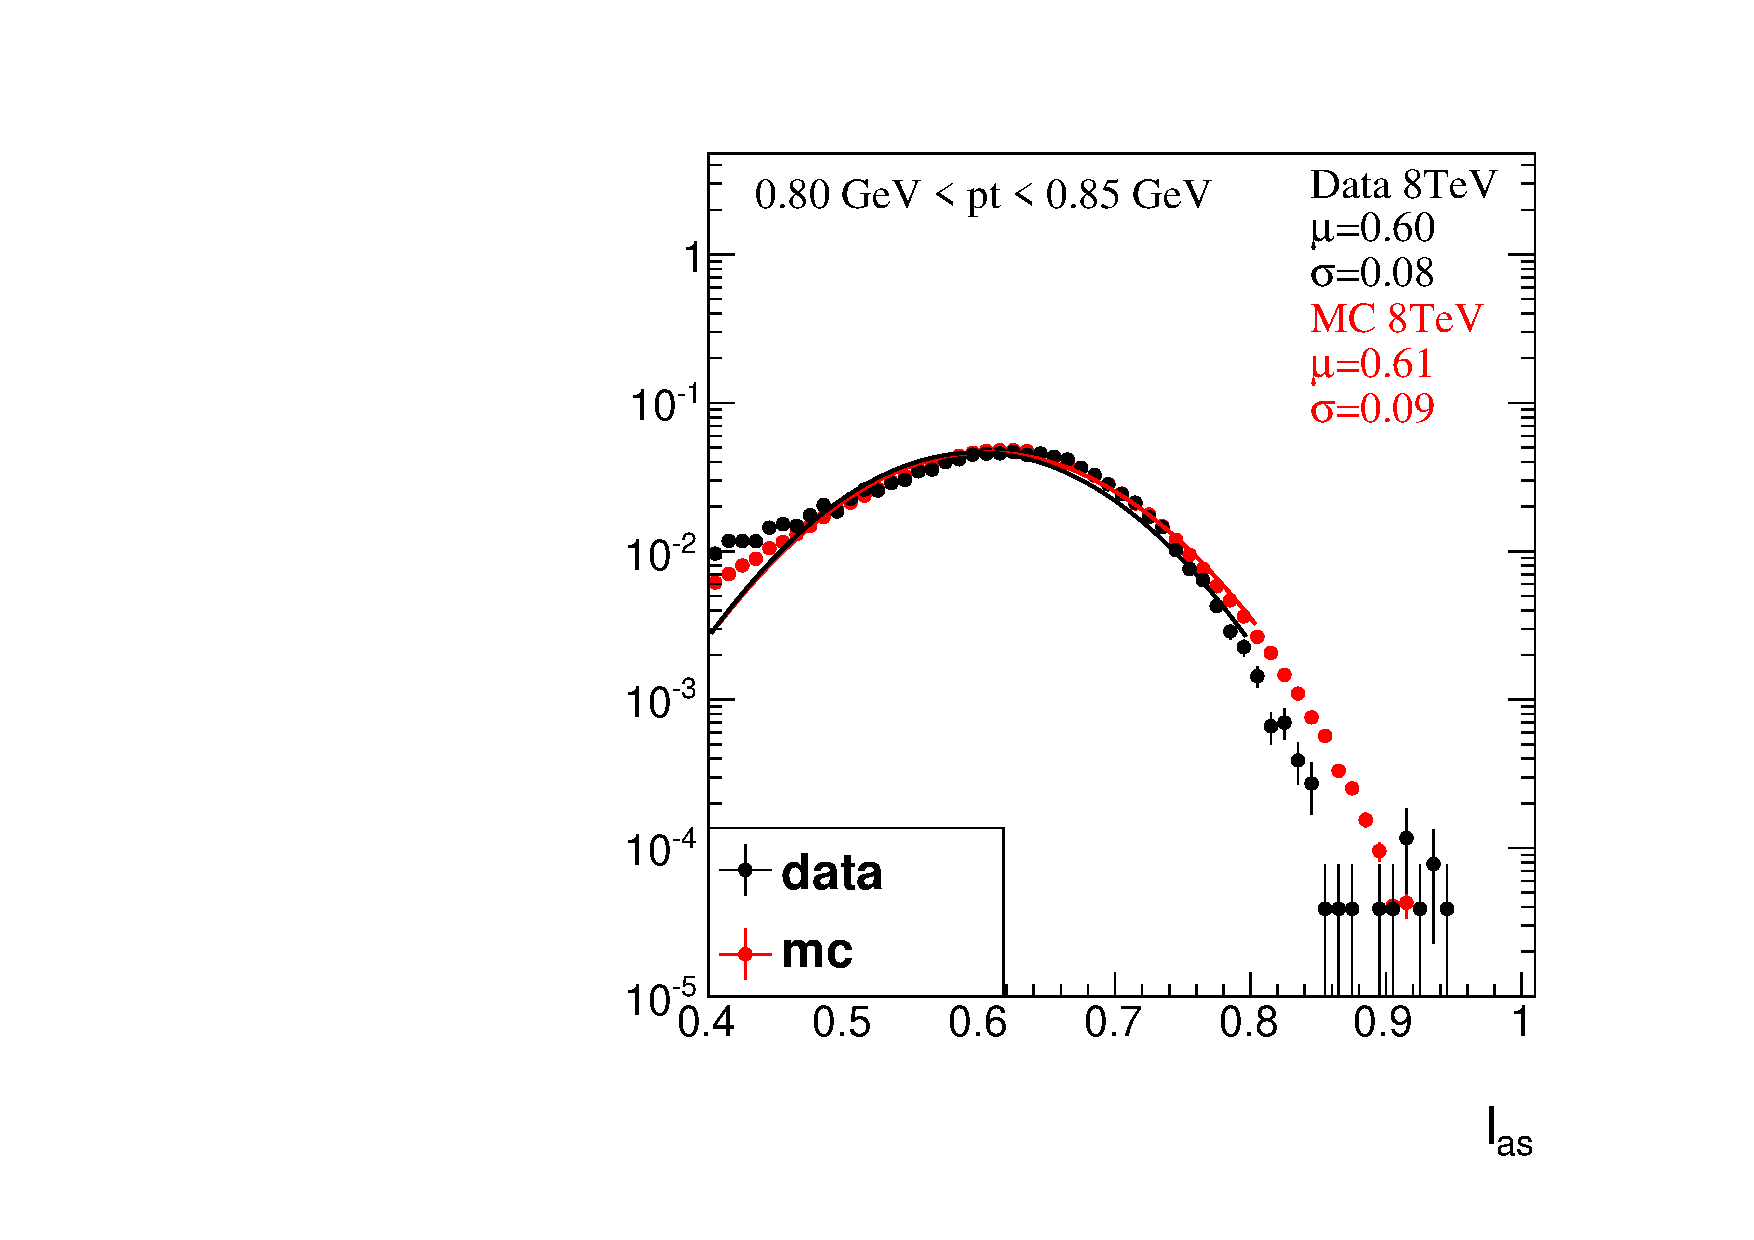
\includegraphics[width=0.49\textwidth]{figures/analysis/Interpretation/hIas_analysis_2015_11_30_ForThesis_ptmin0p80_ptmax0p85.pdf} 
    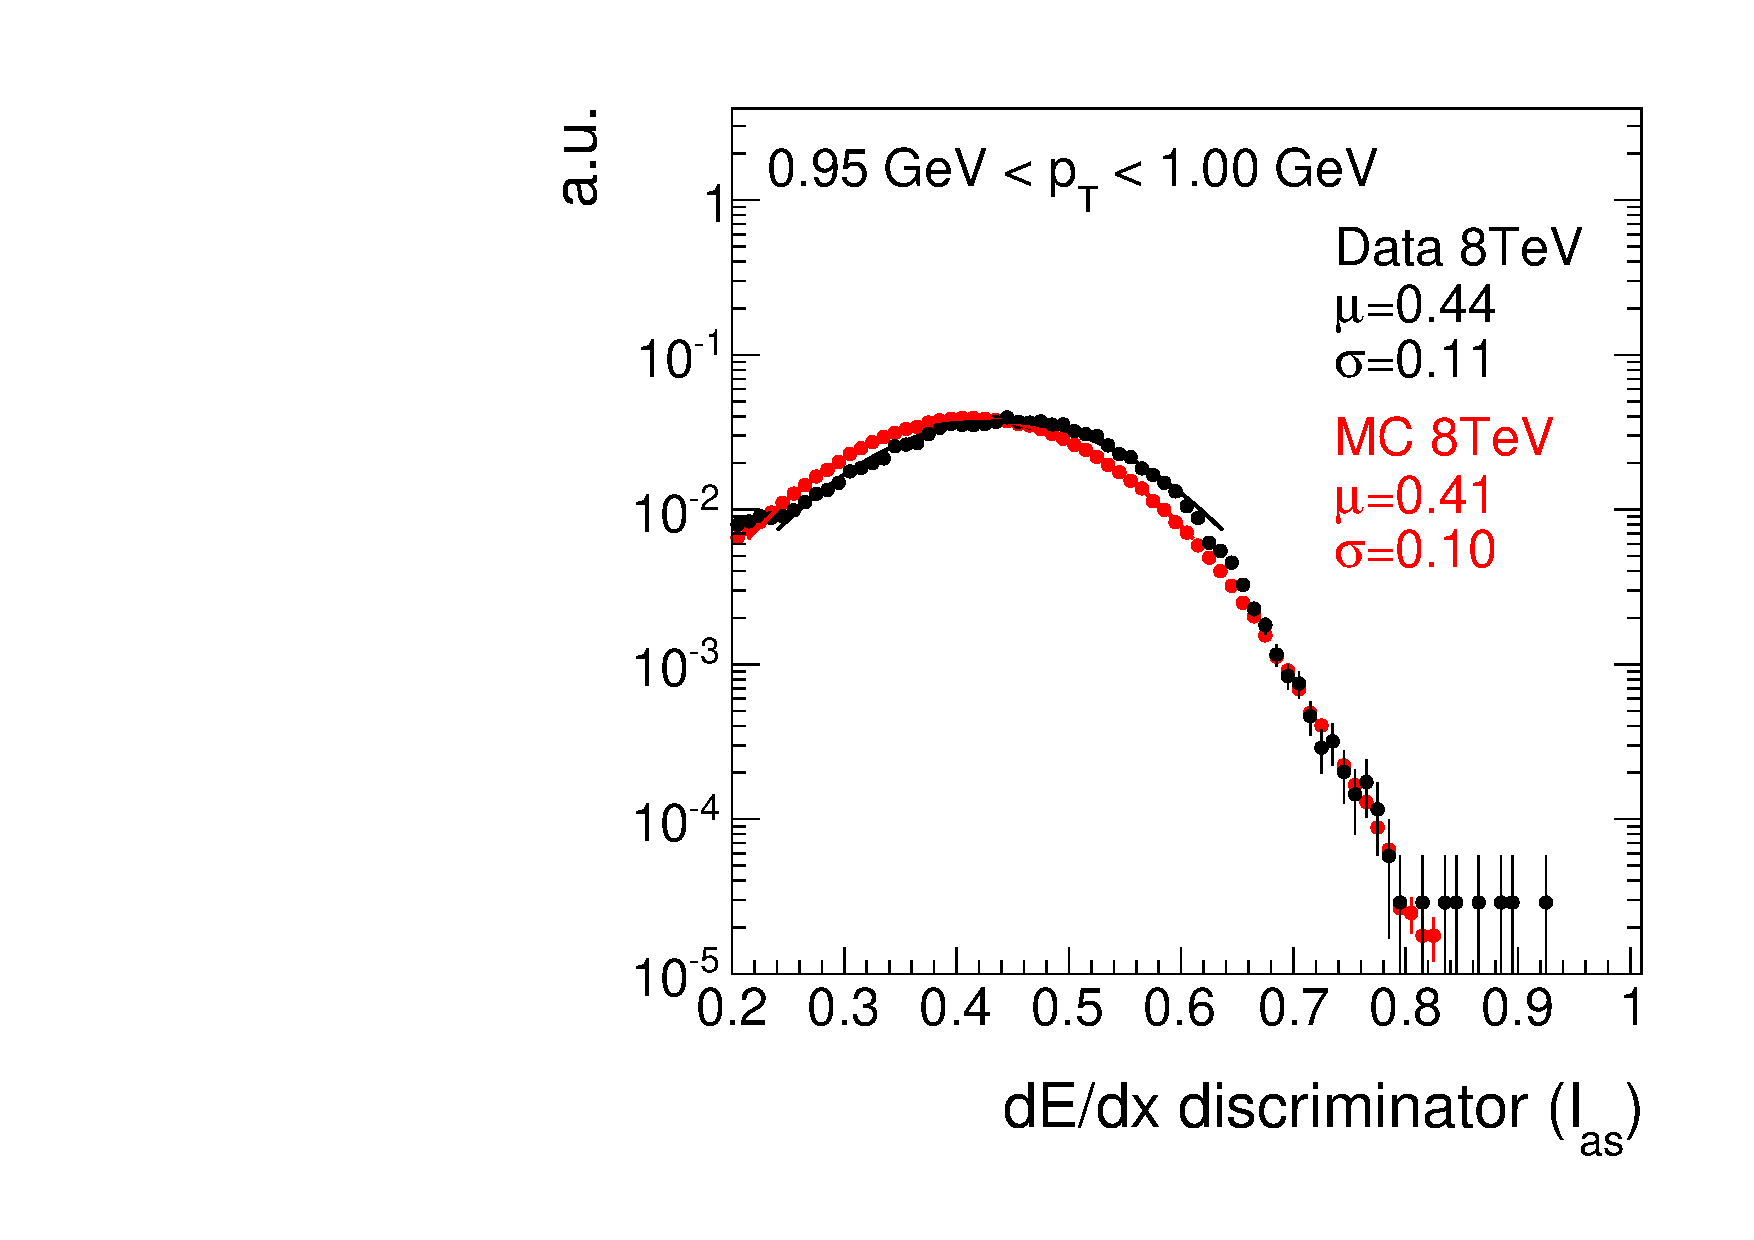
\includegraphics[width=0.49\textwidth]{figures/analysis/Interpretation/hIas_analysis_2015_11_30_ForThesis_ptmin0p95_ptmax1p0.pdf}
  \end{tabular}
  \caption{\ias distribution for slow protons in simulation and observed data for a momentum range of $0.80-0.85\gev$ (left) and $0.95-1.00\gev$ (left).
           For the momentum range of $0.80-0.85\gev$, the proton line is contained between \ias values of $0.4-0.8$, whereas for the momentum range of $0.95-1.00\gev$, the proton line \ias lies between $0.2-0.6$.  }
  \label{fig:IasSlowProtons}
\end{figure} 
The systematic uncertainty is estimated to a value of 6\%.
The size of the systematic uncertainty is also expected to cover the data-simulation difference for minimal ionisation.


\subsection*{Uncertainty on the simulation of the track reconstruction efficiency}
One final source of uncertainty is the simulation of the track reconstruction efficiency.
Possible differences of the reconstruction efficiency in simulation and data can lead to a different signal acceptance.
Differences in the track reconstruction efficiency are especially expected for short tracks.
Therefore, a worst case estimation is done, comparing the track reconstruction efficiency in data and simulation for tracks with a number of hits of three.

In simulation and observed data, well reconstructed muon tracks are selected and all hits after the third hits are removed.
Afterwards the full track reconstruction step is again preformed.
The relative difference of the track reconstruction efficiency in data and simulation ($\epsilon = N_{\text{recon. track with \nhits=3}}/N_{\text{selected muon trks}}$) is taken as systematic uncertainty.
The track reconstruction efficiency is higher in simulation than in data and results in uncertainties between $4.5-6.0\%$.\\


\subsection*{Summary of systematic uncertainties of the simulated signal samples}
All systematic uncertaintes are estimated for all simulated signal samples.
An overview of the range of the uncertainties is given in Table~\ref{tab:SignalSysUnc}.

\renewcommand{\arraystretch}{1.5}
\begin{table}[!h] 
\centering
\caption{Ranges of systematic uncertainties of the simulated signal samples. FIXME: Update this Table with latest uncertainties.}
\label{tab:SignalSysUnc}
\begin{tabular}{|l|c|c|}  
\multicolumn{3}{c}{} \\
\toprule
Uncertainty                             &Min [\%]           &Max [\%]           \\ 
\midrule
Luminosity                              &2.6                &2.6                \\ 
ISR                                     &10.4               &12.6               \\ 
Trigger efficiency                      &2.6                &4.6                \\ 
JES                                     &0.5                &1.1                \\ 
JER                                     &0.1                &0.7                \\ 
PDF                                     &3.0                &4.9                \\ 
Simulation of calorimeter isolation     &0.8                &6.6                \\ 
Simulation of missing middle hits       &1.8                &2.3                \\ 
Simulation of missing inner hits        &3.2                &3.4                \\ 
PU                                      &0.0                &35.9               \\ 
Track reconstruction efficiency         &4.1                &5.1                \\ 
Simulation of Ias                       &6.5                &6.5                \\ 
Theoretical x-section                   &3.4                &8.1                \\ 
\bottomrule
\multicolumn{3}{c}{} \\
\end{tabular}  
\end{table} 

In order to avoid an overestimation of the systematic uncertainties due to limited sizes of the samples (especially for low lifetimes like 1\cm), the corresponding signal sample with longer lifetime (100\cm) is used instead.
This is possible for uncertainty sources, for which the size is not affected by the lifetime of the chargino.
These are the uncertainties in ISR, trigger efficiency, JES, JER and PDF.

It can be seen, that major uncertainties are the simulation of the initial state radiation, of the calorimeter isolation, and of \ias.
The high maximal uncertainty of the pile-up uncertainty is caused by limited statistical precision.

The systematic uncertainties of the simulated signal samples are taken as fully correlated for the four signal bins into account.

%%%%%%%%%%%%%%%%%%%%%%%%%%%%%%%%%%%%%%%%%%%%%%%%%%%%%%%%%%%%%%%%%%%%%%%%%%%%%%%%%%%%%%%%%%%%%%%%%%%%%%%%%%%%%%%%%%%%%%%%%%%%%%%%%%%%%%%%%%%%%%%%%%%%%%%%%%%%%%%%%%%%%%%
%%%%%%%%%%%%%%%%%%%%%%%%%%%%%%%%%%%%%%%%%%%%%%%%%%%%%%%%%%%%%%%%%%%%%%%%%%%%%%%%%%%%%%%%%%%%%%%%%%%%%%%%%%%%%%%%%%%%%%%%%%%%%%%%%%%%%%%%%%%%%%%%%%%%%%%%%%%%%%%%%%%%%%%
%\section{Correlation of systematic uncertainties}
%In order to combine the four different signal regions, a specification of the size of correlations between the systematic uncertay needs to be addresses.
%\subsection*{Background correlations}
%\subsection*{Signal correlation}
%%%%%%%%%%%%%%%%%%%%%%%%%%%%%%%%%%%%%%%%%%%%%%%%%%%%%%%%%%%%%%%%%%%%%%%%%%%%%%%%%%%%%%%%%%%%%%%%%%%%%%%%%%%%%%%%%%%%%%%%%%%%%%%%%%%%%%%%%%%%%%%%%%%%%%%%%%%%%%%%%%%%%%%
%%%%%%%%%%%%%%%%%%%%%%%%%%%%%%%%%%%%%%%%%%%%%%%%%%%%%%%%%%%%%%%%%%%%%%%%%%%%%%%%%%%%%%%%%%%%%%%%%%%%%%%%%%%%%%%%%%%%%%%%%%%%%%%%%%%%%%%%%%%%%%%%%%%%%%%%%%%%%%%%%%%%%%%
\section{Statistical Methods/ Limit setting}
This section is a small interlude to give a short introduction into the methods and techniques of the exclusion of theoretical models used in this analysis.
For a detailed and pedagigical introduction to the methods, it is refered to~\cite{bib:Ott_Thesis}.

In this analysis the exclusion of the underlying theoretical model is achieved with the \CLs method~\cite{bib:CLS_1999,bib:CLS_2000,bib:CLS_2002}.
The \CLs method was developed for the Higgs searches at LEP in order not to overestimate the exclusion power of a result when an  underfluctuation of the Standard Model expectation occurs.
\CLs is defined as the confidence level for the background plus signal hypothesis devided by the confidence level for the background hypothesis only
\begin{equation*}
\CLs = \frac{\CLsb}{\CLb}.
\end{equation*}
The confidence level CL is defined as the probability to observe less than or equal the number of observed events P($n<n_{\text{obs}}$) for a given background (or background+signal) hypothesis.
In general, the considered distribution can be any constructed test statistics $Q$ and is not necessarily the distribution in the number of events.
However, For Poissonian statistics it leads to the following expressions for \CLsb and \CLb for one signal region
\begin{equation*}
\begin{split}
\CLsb &= \text{Poisson}\left( n<n_{\text{obs}} |\lambda = b+\mu\cdot s   \right),\\
\CLb  &= \text{Poisson}\left( n<n_{\text{obs}} |\lambda = b   \right),
\end{split}
\end{equation*}
where $\lambda$ is the mean of the poisson distribution and $\mu$ is the signal strength.
The signal strength $\mu$ is a measure for the size of the signal cross section.

In order to include systematic uncertainties, the background expectation $b$ or the signal expectation $\mu\cdot s$ are varied within a Gaussian distribution with a width estimated as the 1-$\sigma$ uncertainty and a mean of zero.
For one source of systematic uncertainty on the background, this leads to the following expressions for \CLsb and \CLb
\begin{equation*}
\begin{split}
\CLsb &= \text{Poisson}\left( n<n_{\text{obs}} |\lambda = b \cdot (1+\delta_b)+\mu\cdot s   \right) \text{Gauss}\left(\delta_b|\text{mean}=0, \sigma = \delta_b\right),\\
\CLb  &= \text{Poisson}\left( n<n_{\text{obs}} |\lambda = b \cdot (1+\delta_b)   \right) \text{Gauss}\left(\delta_b|\text{mean}=0, \sigma = \delta_b\right),
\end{split}
\end{equation*}
These expressions can be generalised for more than one signal region and more than one systematic uncertainty~\cite{bib:Ott_Thesis}.
A model is considered as excluded at a 95\% confidence level when \CLs is smaller than 5\%.



In this search, the systematic uncertainties on the background expectation are taken as (un-)correlated according to Table~\ref{tab:BkgSysUncCorr}.
The systematic uncertainties on the expected signal yields are considered fully correlated.

\renewcommand{\arraystretch}{1.5}
\begin{table}[!h] 
\centering
\caption{Correlation of systematic and statistical uncertainties between the four different signal regions.}
\label{tab:BkgSysUncCorr}
\begin{tabularx}{\textwidth}{|X|X|X|X|X|}  
\multicolumn{5}{c}{} \\
\toprule 
                                        & Fakes                        & Taus                          & Electrons                      & Muons                       \\ 
\midrule
Statistical uncertainty                 &0\% correlated                & 100\% for same bins in \ias   & 0\% correlated                 & 100\% for same bins in \ias \\
\midrule
Leptonic scale factor uncertainty       & \centering -                 & 100\% for same bins in \ias   & 100\% for same bins in \ias    & 100\% for same bins in \ias \\
\midrule
Fake rate  uncertainty                  & 100\% for same bins in \ias  &  -                            &  -                             &  -                          \\
\midrule
Ias uncertainty                         &0\% correlated                & 100\% for same bins in \pt    & 100\% for same bins in \pt     &  100\% for same bins in \pt \\
\bottomrule
\multicolumn{5}{c}{} \\
\end{tabularx}  
\end{table} 



%%%%%%%%%%%%%%%%%%%%%%%%%%%%%%%%%%%%%%%%%%%%%%%%%%%%%%%%%%%%%%%%%%%%%%%%%%%%%%%%%%%%%%%%%%%%%%%%%%%%%%%%%%%%%%%%%%%%%%%%%%%%%%%%%%%%%%%%%%%%%%%%%%%%%%%%%%%%%%%%%%%%%%%
%%%%%%%%%%%%%%%%%%%%%%%%%%%%%%%%%%%%%%%%%%%%%%%%%%%%%%%%%%%%%%%%%%%%%%%%%%%%%%%%%%%%%%%%%%%%%%%%%%%%%%%%%%%%%%%%%%%%%%%%%%%%%%%%%%%%%%%%%%%%%%%%%%%%%%%%%%%%%%%%%%%%%%%
\section{Exclusion limits}

The search for highly ionising short tracks is interpreted within SUSY models with wino-like chargino and neutralinos.
As explained in the previous section, the exclusion is done with the help of the \CLs method.
As production channels, chargino pair production and chargino neutralino production are taken into account. 
The corresponding cross sections can be found in Table~\ref{tab:SignalCrossSections}.
The exclusion limits are derived with the Combine framework~\cite{bib:CMS:Combine} developed for the Higgs searches at CMS.
The systematic uncertainties on the background and the signal yields  are modelled with log-normal distributions, whereas the statistical uncertainties on the background are modelled with a gamma distributions.
The log-normal distribution is used rather than a normal distribution to ensure that the prediction cannot become negative.
The gamma distribution is well suited for statistical uncertainties arising from limited statistical precision in control regions or in simulated samples.

In total, 37 different lifetimes for every mass point are considered, leading to 37 different exclusion limits.
Four exemplary exclusion limits are shown in Fig.~\ref{fig:1dLimits}, the full set of exclusion limits can be found in Appendix~\ref{FIXME}.

\begin{figure}[!h]
  \centering 
  \begin{tabular}{c}
    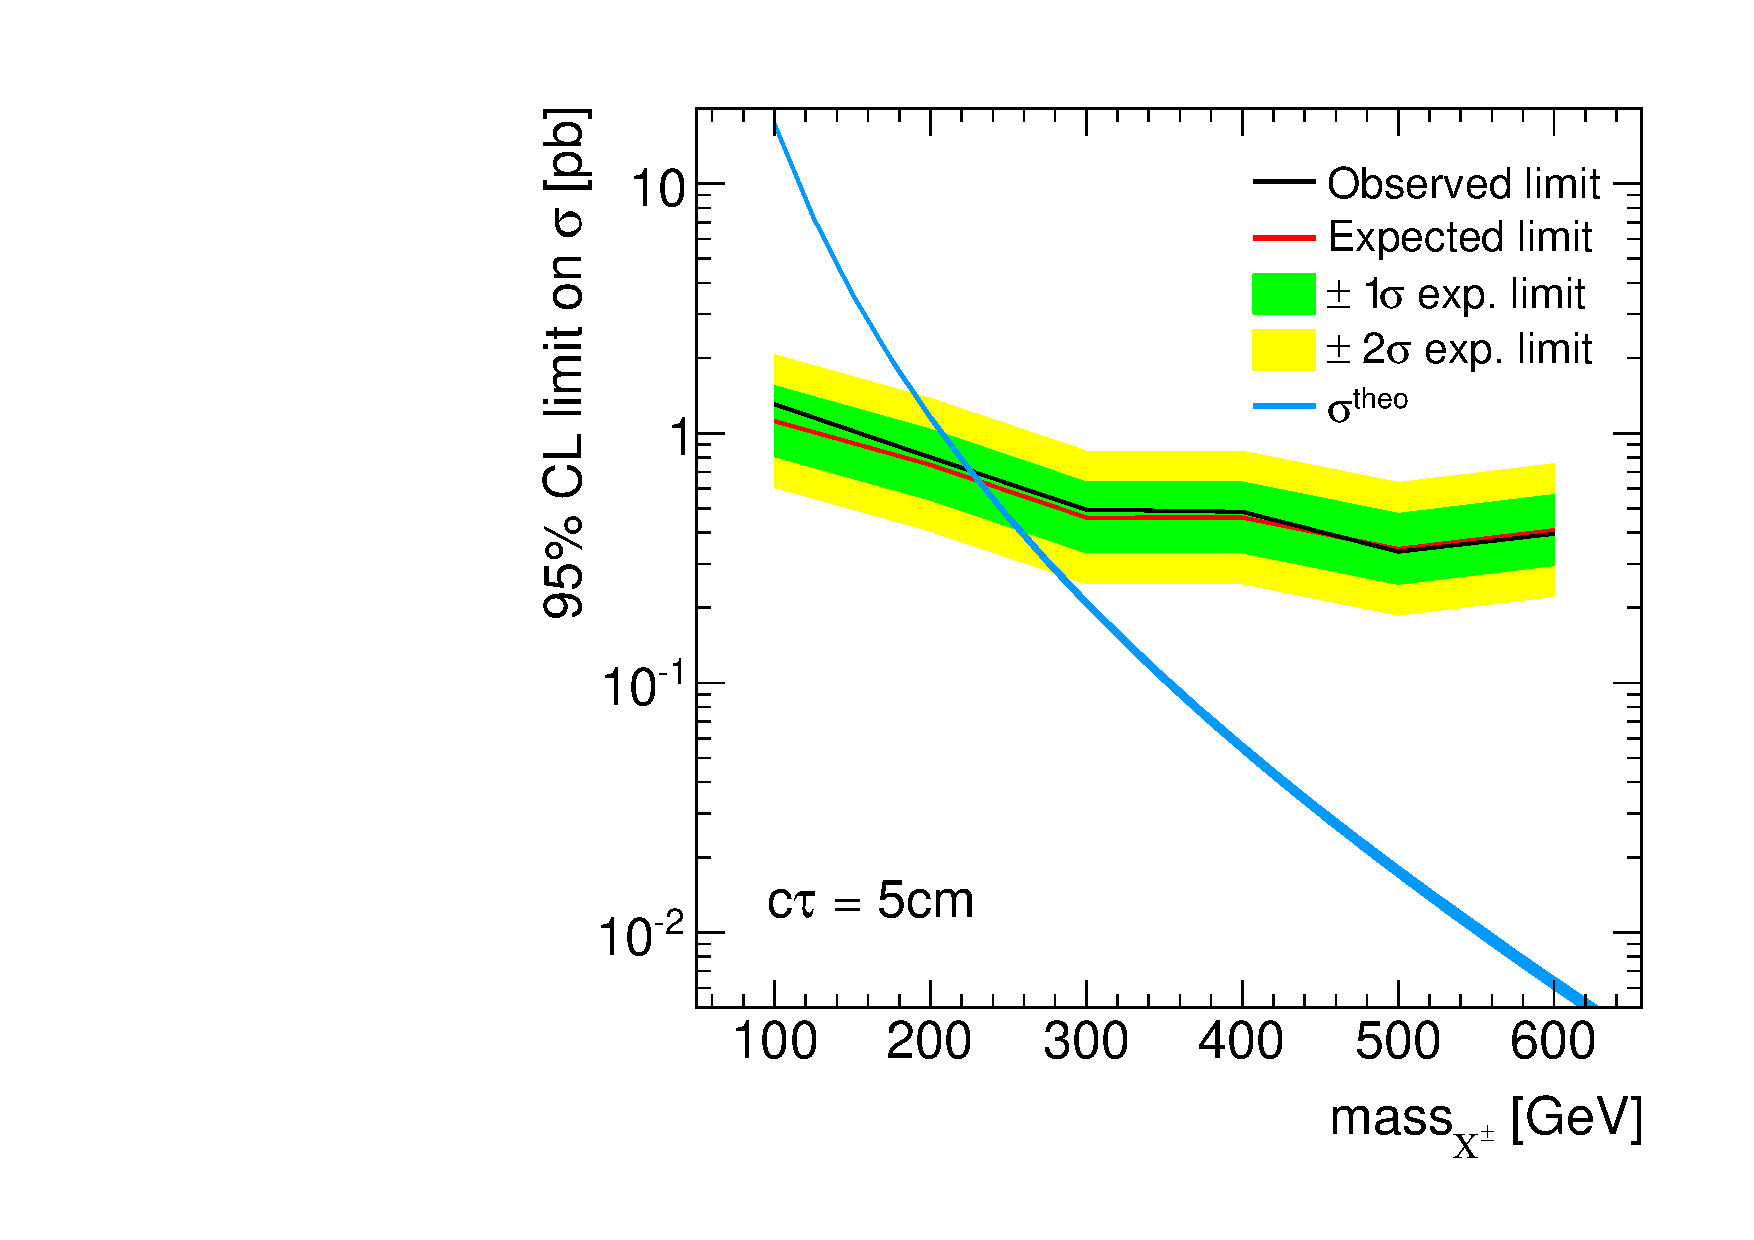
\includegraphics[width=0.49\textwidth]{figures/analysis/Interpretation/ExclusionLimits/LimitPlot_ctau5cm.pdf} 
    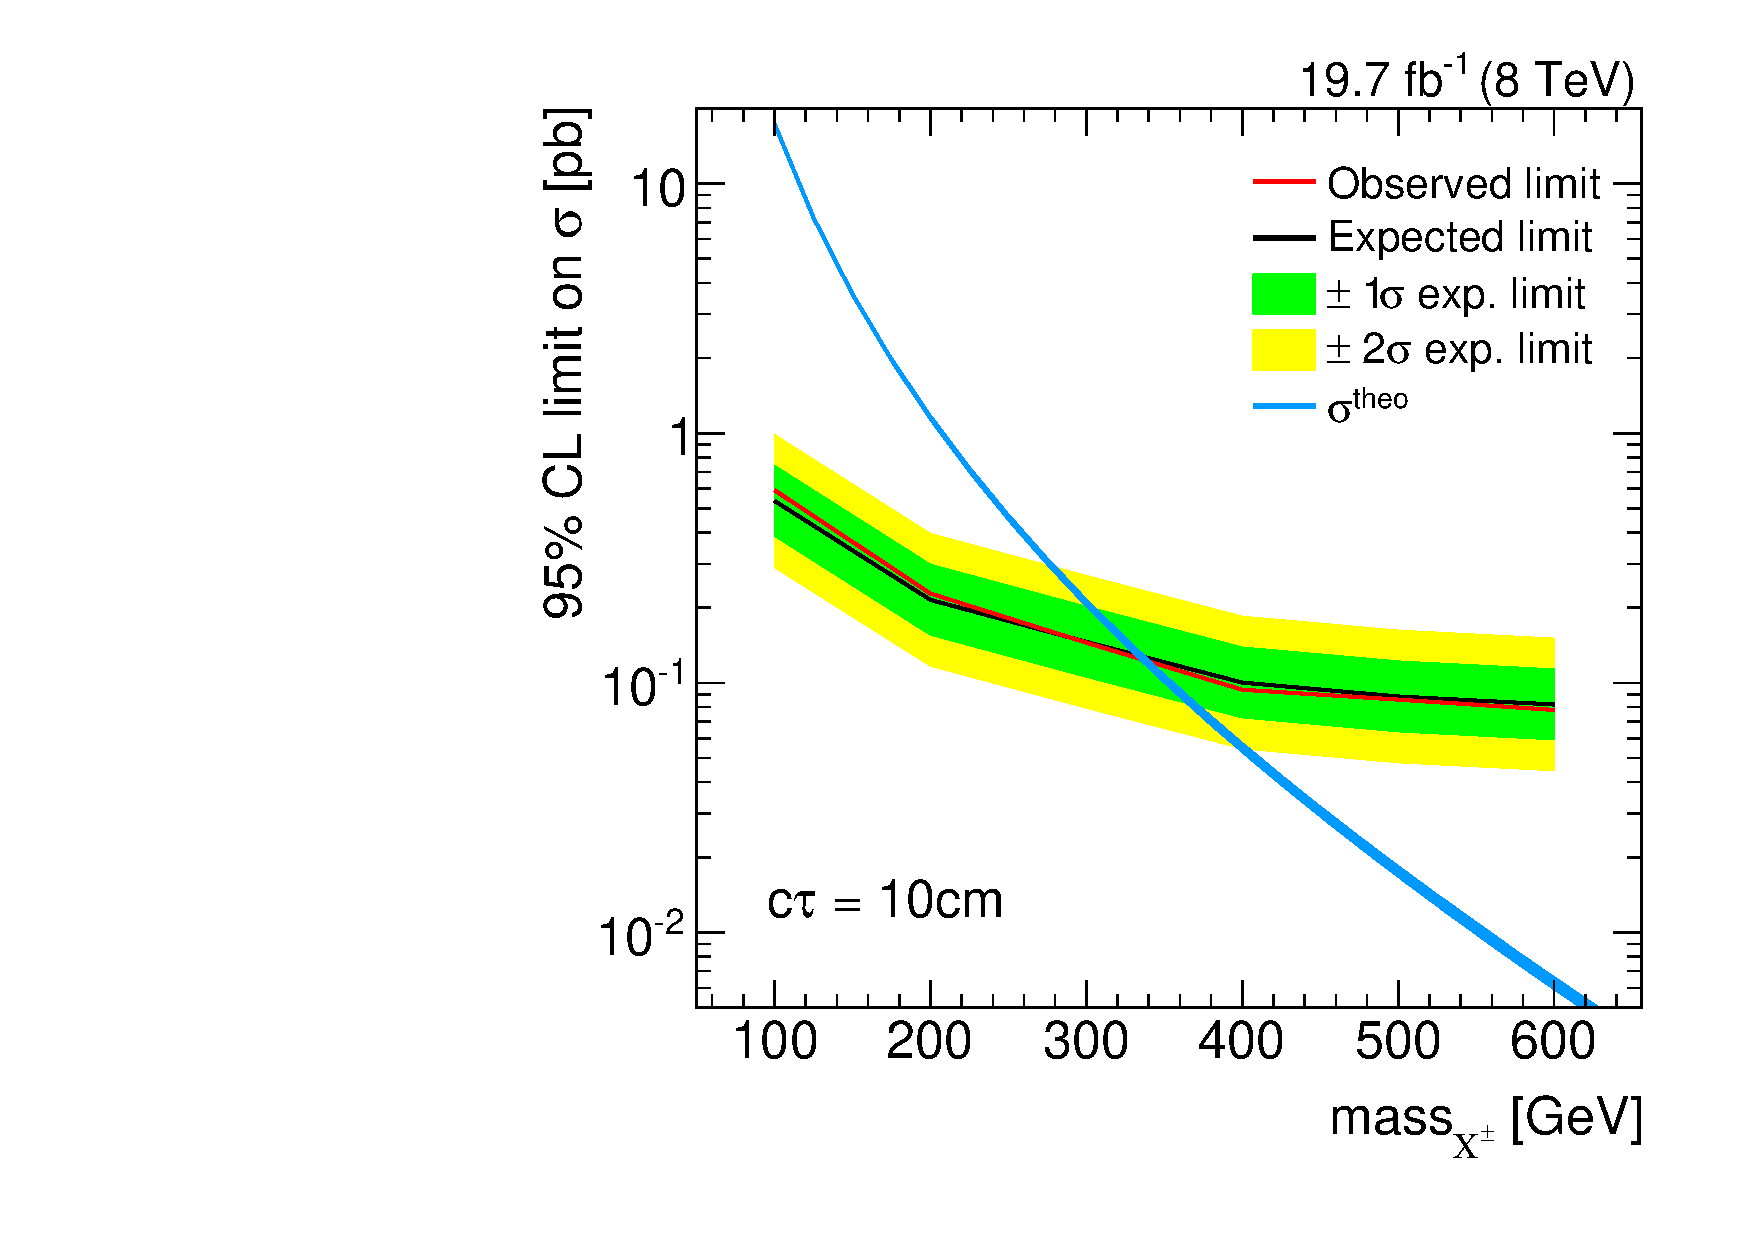
\includegraphics[width=0.49\textwidth]{figures/analysis/Interpretation/ExclusionLimits/LimitPlot_ctau10cm.pdf} \\
    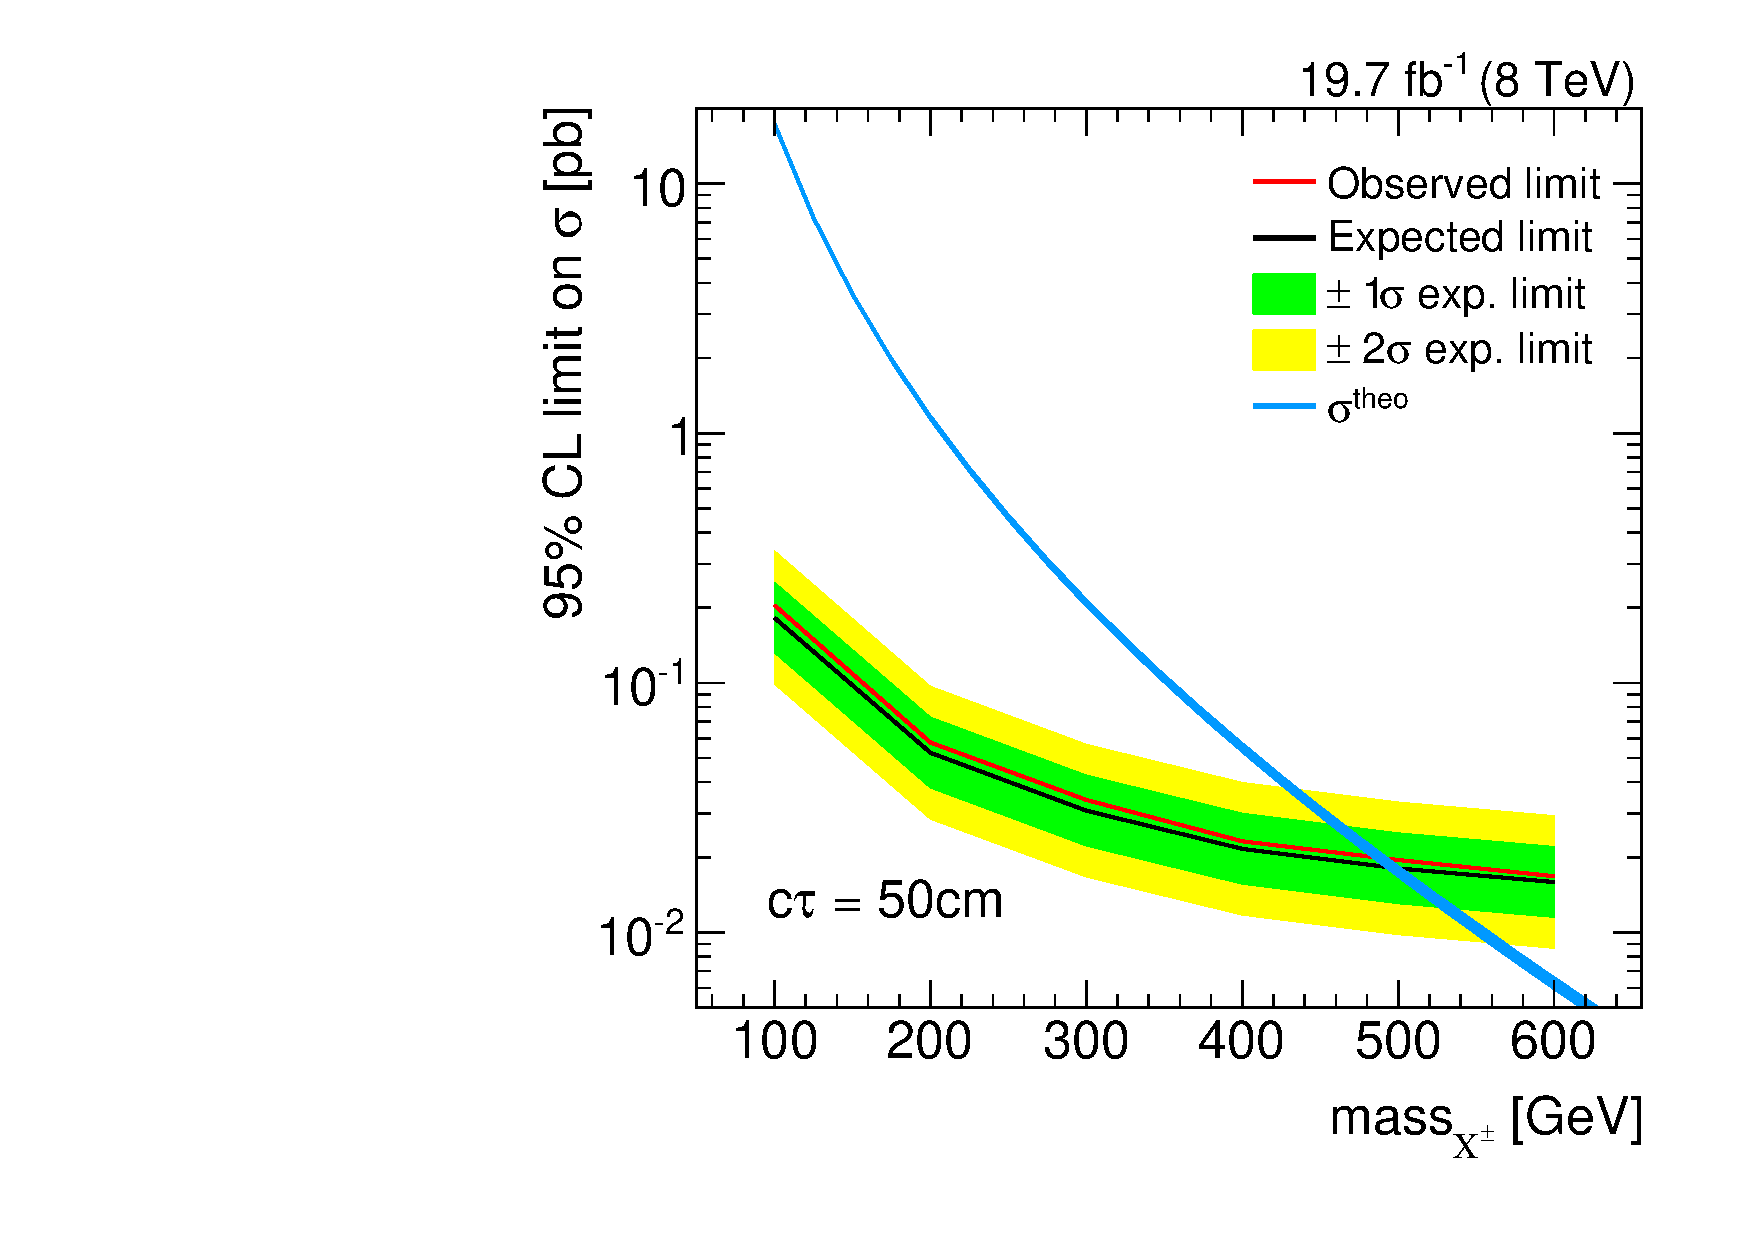
\includegraphics[width=0.49\textwidth]{figures/analysis/Interpretation/ExclusionLimits/LimitPlot_ctau50cm.pdf} 
    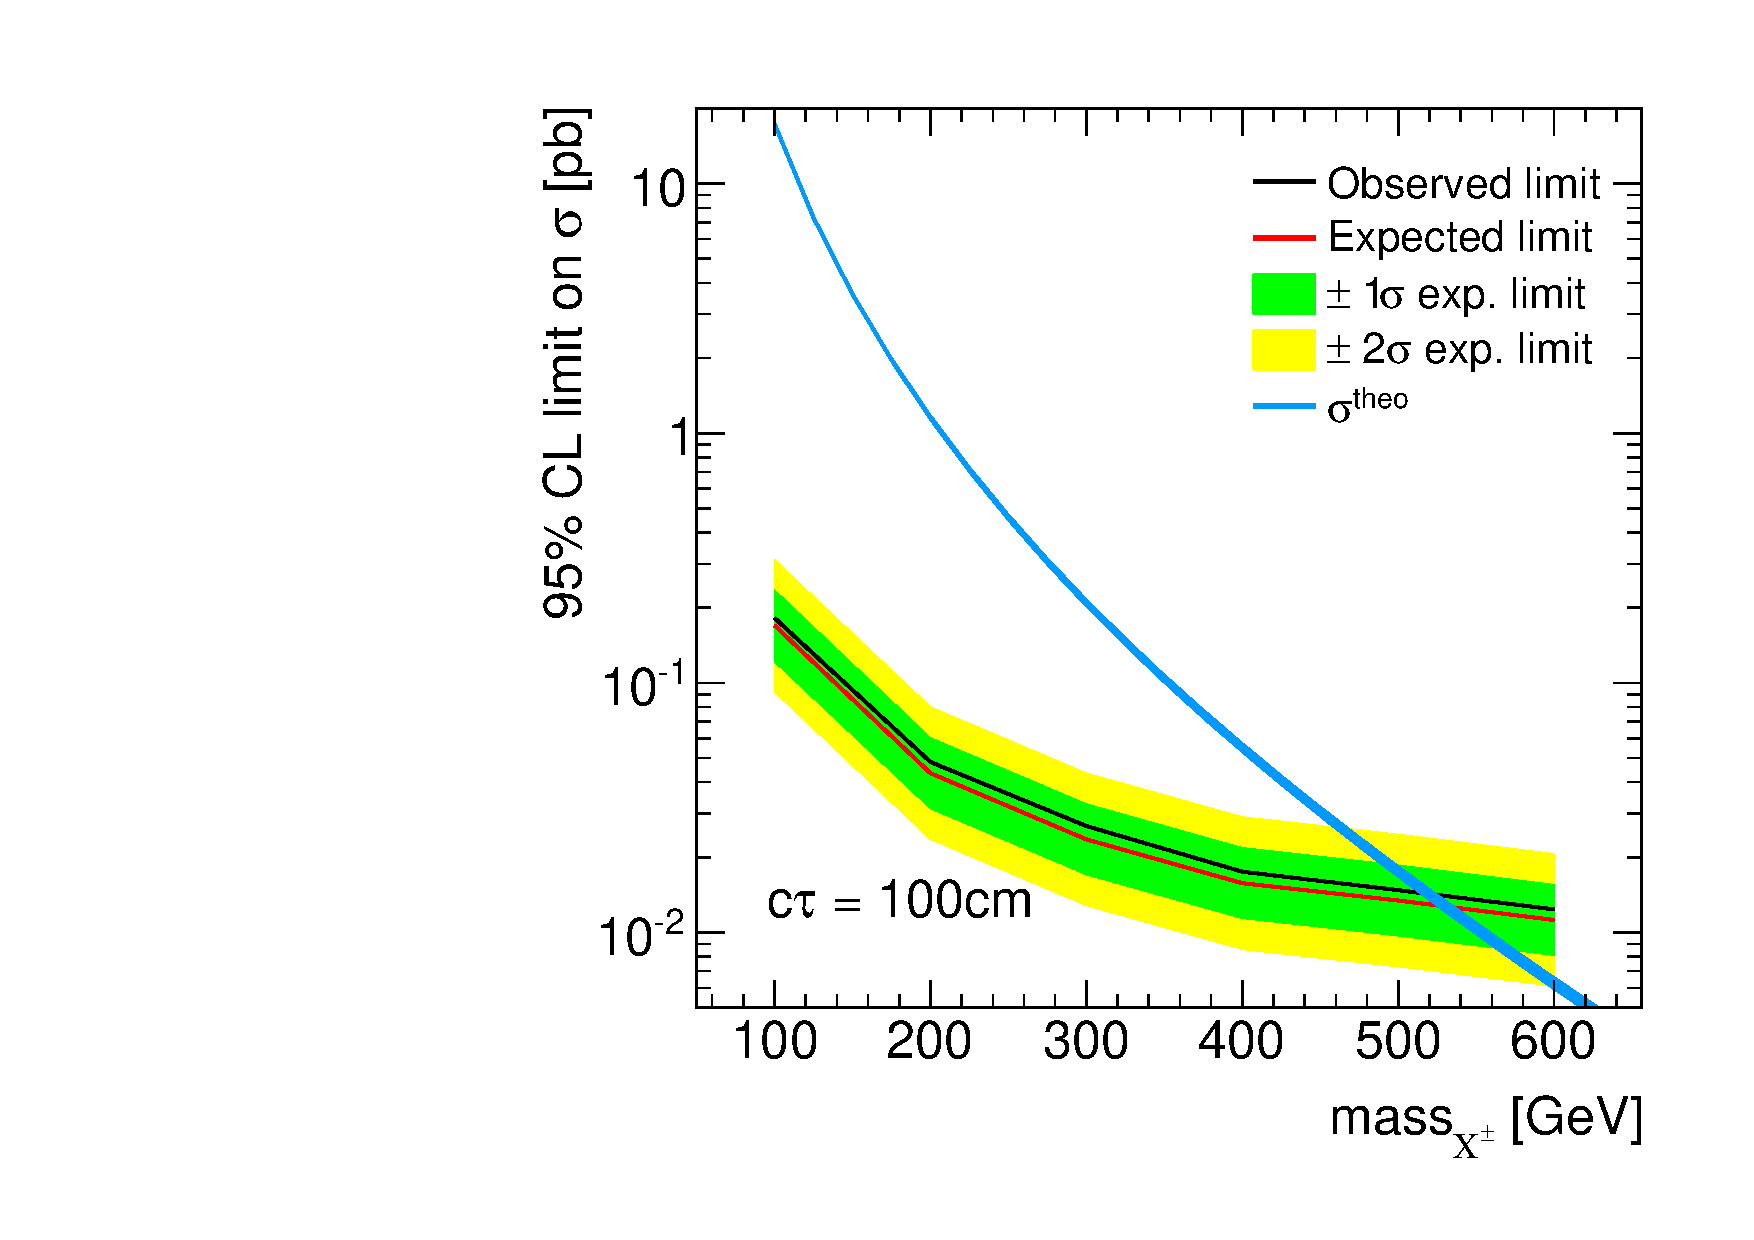
\includegraphics[width=0.49\textwidth]{figures/analysis/Interpretation/ExclusionLimits/LimitPlot_ctau100cm.pdf} 
  \end{tabular}
  \caption{Four different exclusion limits for charginos with mean lifetimes of 5\cm (top left), 10\cm (top right), 50\cm (bottom left), 100\cm (bottom right).
           The red line gives th expected 95\% upper cross-section limit with the 1-$\sigma$ (green band) and 2-$\sigma$ (yellow band).
           The black line is the observed limit.
           The signal cross section is depicted as dark green line. 
           SUSY models can be excluded with a 95\% confidence when the signal cross section is large as the 95\% observed upper limit on the cross section.}
  \label{fig:1dLimits}
\end{figure} 
Due to the higher cross sections for lower masses the exclusion is stronger is the low chargino mass region.
A 2-dimensional exclusion limit in the chargino lifetime/mass paramater space is shown in Fig.~\ref{FIXME}.
\begin{figure}[!h]
  \centering 
  \begin{tabular}{c}
    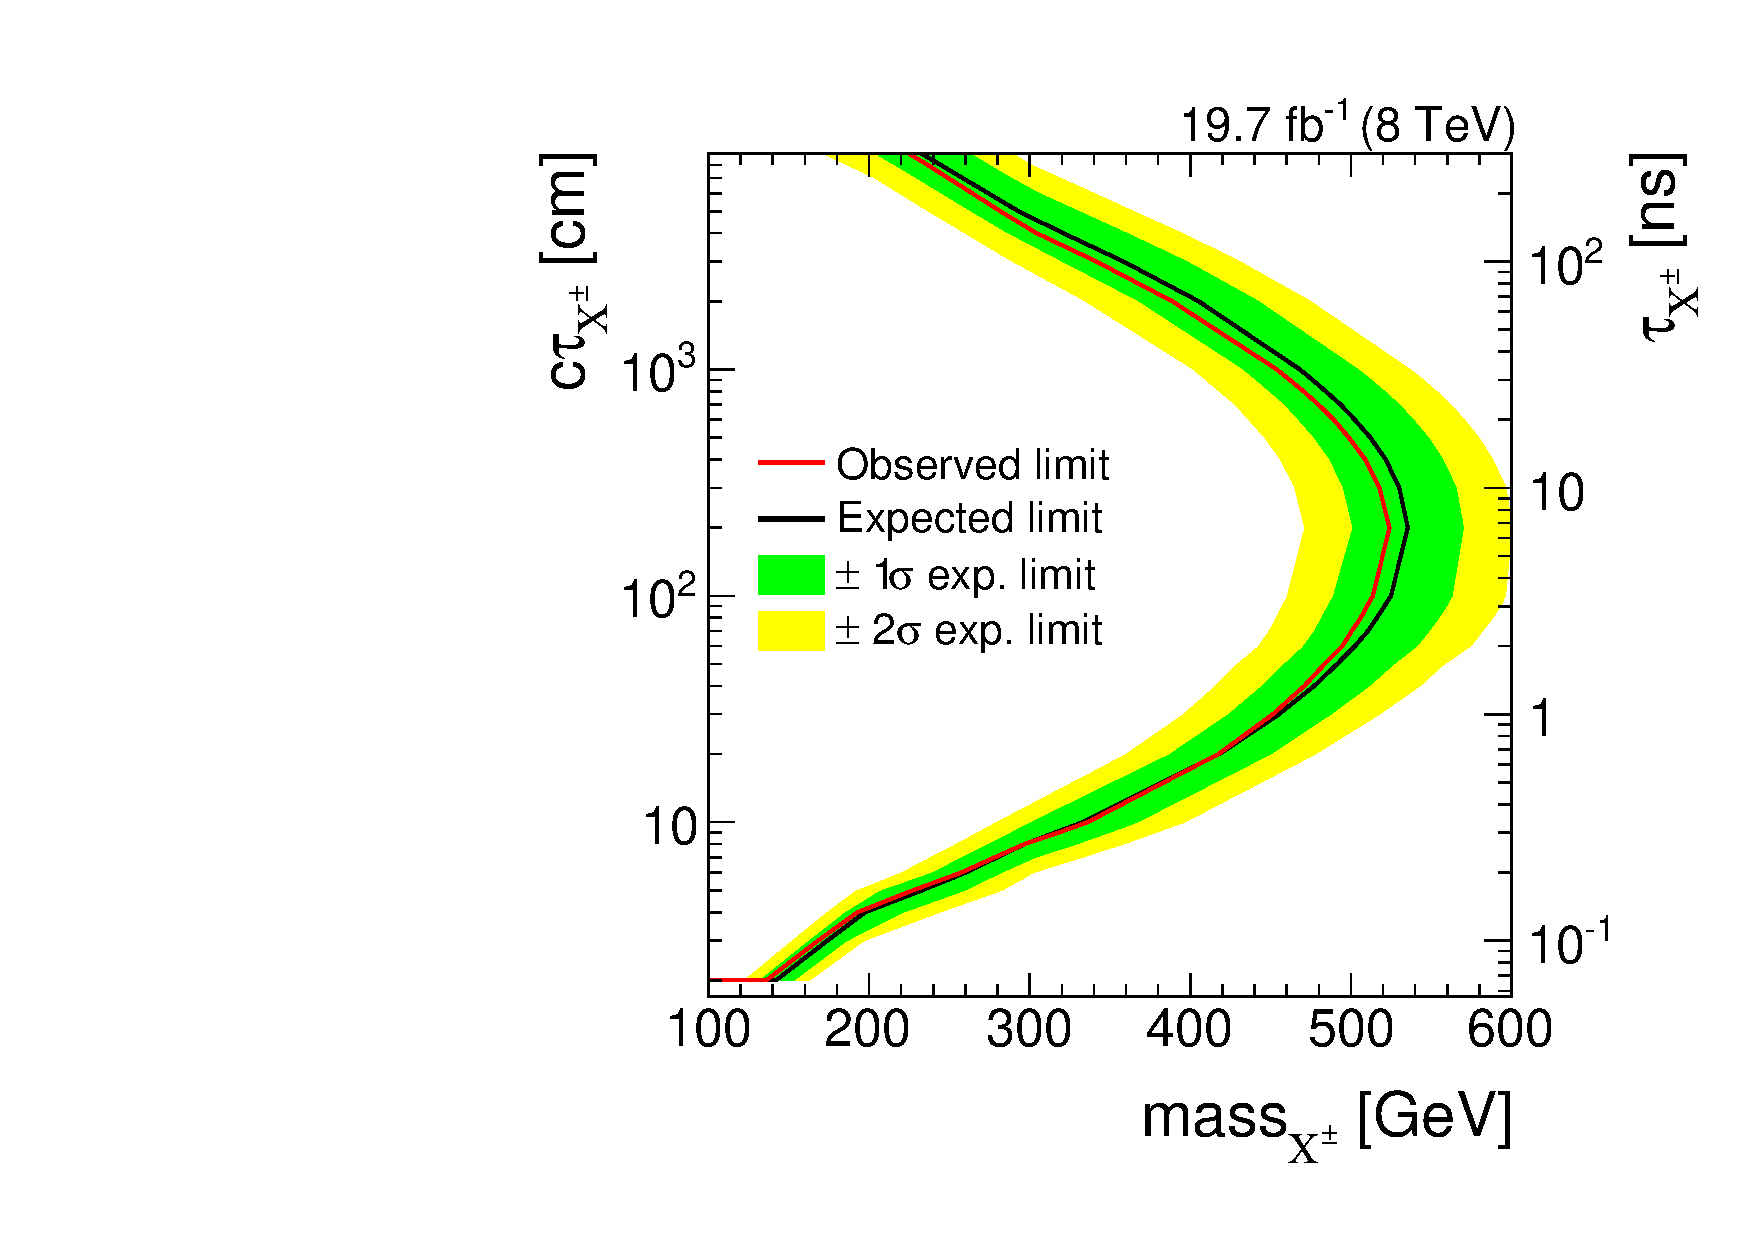
\includegraphics[width=0.69\textwidth]{figures/analysis/Interpretation/ExclusionLimits/LimitPlot_2d_log_cm.pdf} 
  \end{tabular}
  \caption{Excluded regions in the mass versus lifetime space.
           Excluded models are all lying within the contour line.
          1 sigma}
  \label{fig:1dLimits}
\end{figure} 
Signal models up to a mass of $\sim FIXME \gev$ with lifetimes around FIXME can be excluded.
Signal models up to a mass of $\sim FIXME \gev$ with lifetimes around FIXME can be excluded.
Signal models up to a mass of $\sim FIXME \gev$ with lifetimes around FIXME can be excluded.
Signal models up to a mass of $\sim FIXME \gev$ with lifetimes around FIXME can be excluded.
Signal models up to a mass of $\sim FIXME \gev$ with lifetimes around FIXME can be excluded.
Signal models up to a mass of $\sim FIXME \gev$ with lifetimes around FIXME can be excluded.
Signal models up to a mass of $\sim FIXME \gev$ with lifetimes around FIXME can be excluded.
Signal models up to a mass of $\sim FIXME \gev$ with lifetimes around FIXME can be excluded.
Signal models up to a mass of $\sim FIXME \gev$ with lifetimes around FIXME can be excluded.
Signal models up to a mass of $\sim FIXME \gev$ with lifetimes around FIXME can be excluded.
Signal models up to a mass of $\sim FIXME \gev$ with lifetimes around FIXME can be excluded.
Signal models up to a mass of $\sim FIXME \gev$ with lifetimes around FIXME can be excluded.
Signal models up to a mass of $\sim FIXME \gev$ with lifetimes around FIXME can be excluded.
Signal models up to a mass of $\sim FIXME \gev$ with lifetimes around FIXME can be excluded.
Signal models up to a mass of $\sim FIXME \gev$ with lifetimes around FIXME can be excluded.
Signal models up to a mass of $\sim FIXME \gev$ with lifetimes around FIXME can be excluded.
Signal models up to a mass of $\sim FIXME \gev$ with lifetimes around FIXME can be excluded.
Signal models up to a mass of $\sim FIXME \gev$ with lifetimes around FIXME can be excluded.


%%%%%%%%%%%%%%%%%%%%%%%%%%%%%%%%%%%%%%%%%%%%%%%%%%%%%%%%%%%%%%%%%%%%%%%%%%%%%%%%%%%%%%%%%%%%%%%%%%%%%%%%%%%%%%%%%%%%%%%%%%%%%%%%%%%%%%%%%%%%%%%%%%%%%%%%%%%%%%%%%%%%%%%
\chapter{Discussion and conclusion}
\label{sec:Discussion}

\begin{itemize}
\item Earlier limits could verified and slightly improved in mass regions between 300-400 to 50\gev
\item The inclusion of ias discriminatior shows good sensitivty increase of 100\% ...
\item further improvements throudh bla bla
\end{itemize}
